\def\docversion{2}
\documentclass{book}
\usepackage{solrexbook}[2007/08/30]


% 设置 PDF 文件属性
\hypersetup {
    pdftitle={使用开源软件-自己动手写操作系统},
    pdfauthor={杨文博}%,
}

\makeindex

\begin{document}

\def\BookName{使用开源软件-自己动手写操作系统} 

\pagestyle{empty}
\begin{center}
\Huge 使用开源软件

\CJKfamily{hei}\fontsize{48}{52}\selectfont 自己动手写操作系统

\CJKfamily{song}
\bf\sc\Huge Write Your Own OS with\\ Free and Open Source Software

\it\LARGE Alpha Edition

\end{center}
\vskip 1cm
\begin{figure}[htbp]
 \centering

\includegraphics[width=0.8\textwidth]{cover}
\end{figure}

\noindent\makebox[\textwidth][r]{\bf\LARGE 杨文博~~著}
\noindent\makebox[\textwidth][l]{\normalsize \today~~\currenttime~~Revision~~\docversion}
\clearpage

\begin{lined}{\textwidth}\vspace{2ex}
\begin{center}
\bf\Large 版权声明
\end{center}
\vspace{2ex}
\end{lined}

\normalsize
本文遵从\href{http://creativecommons.org/licenses/by-nc-sa/2.5/cn/}{署名-非商业性使用-相同方式共享~2.5~中国大陆创作共享协议}。
\vskip 1cm
\noindent
\large 您可以自由:
\normalsize
\begin{itemize}
\item 复制、发行、展览、表演、放映、广播或通过信息网络传播本作品。
\end{itemize}

\noindent
\large 惟须遵守下列条件:
\normalsize
\begin{itemize}
\item{署名.} 您必须按照作者或者许可人指定的方式对作品进行署名。
\item{非商业性使用.} 您不得将本作品用于商业目的。
\item{相同方式共享.} 如果您改变、转换本作品或者以本作品为基础进行创作,您只能采用与本协议相同的许可协议发布基于本作品的演绎作品。
\item 对任何再使用或者发行,您都必须向他人清楚地展示本作品使用的许可协议条款。
\item 如果得到著作权人的许可,您可以不受任何这些条件的限制。
\item Nothing in this license impairs or restricts the author's moral rights.
\end{itemize}
\vskip 1cm
\normalsize
\begin{center}
您的合理使用以及其他权利不受上述规定的影响。

这是一份普通人可以理解的\href{http://creativecommons.org/licenses/by-nc-sa/2.5/cn/legalcode}{法律文本(许可协议全文)}的概要。 
\end{center}

\vspace{5ex}

\begin{lined}{\textwidth}\vspace{2ex}
\begin{center}
相关链接
\end{center}
\vspace{2ex}
\end{lined}

您可以在本书~\href{http://share.solrex.cn/WriteOS/}{官方网站}~: ~\url{http://share.solrex.cn/WriteOS/}~下载到本书的最新版本和附带的全部程序源代码。

由于此版本非最终发布版,如果您对本书感兴趣,请关注作者在其~\href{http://blog.solrex.cn/articles/category/cs/opensource/writeos}{博客}~(~\url{http://blog.solrex.cn}~)~上发布的更新公告。

\cleardoublepage

\pagecolor[rgb]{.9,.9,.9}
\pagestyle{fancy}
\fancyhf{}
\fancyhead[LE,RO]{\small\bfseries\thepage}
\fancyhead[LO]{\small\bfseries\nouppercase{\leftmark}}
\fancyhead[RE]{\small\bfseries\nouppercase{\rightmark}}
\renewcommand{\headrulewidth}{0pt}

\titleformat{\chapter}[display]
{\bfseries\Large}
{\filleft\MakeUppercase{\chaptertitlename} \Huge\thechapter}
{4ex}
{\titlerule
\vspace{2ex}%
\filright}
[\vspace{2ex}%
\titlerule]

\frontmatter
\chapter{写在前面的话} \label{fore}


\begin{kaitext}

本书起源于中国电子工业出版社出版的一本书:《自己动手写操作系统》(于渊著)。我对《自己动手写操作系统》这本书中使用商业软件做为演示平台比较惊讶,因为不是每个人都买得起正版软件的,尤其是穷学生。我想《自》所面向的主要受众也应该是学生,那么一本介绍只有商业软件才能实现的编程技巧的书将会逼着穷学生去使用盗版,这是非常罪恶的行为~\frownie。

由于本人是一个~Linux~用户,一个开源软件的拥护者,所以就试着使用开源软件实现这本书中的所有~demo~,并在\href{http://blog.solrex.cn}{自己的博客}上进行推广。后来我觉得,为什么我不能自己写本书呢?这样我就能插入漂亮的插图,写更详尽的介绍而不怕篇幅过长,更容易让读者接受也更容易传播,所以我就开始写这本《~\BookName~》。

定下写一本书的目标毕竟不像写一篇博客,我将尽量详尽的介绍我使用的方法和过程,以图能让不同技术背景的读者都能通畅地完成阅读。但是自己写并且排版一本书不是很轻松的事情,需要耗费大量时间,所以我只能抽空一点一点的将这本书堆砌起来,这也是您之所以在本页上方看到本书版本号的原因~\smiley。

本书的最终目标是成为一本大学“计算机操作系统”课程的参考工具书,为学生提供一个~step by step~的引导去实现一个操作系统。这不是一个容易实现的目标,因为我本人现在并不自信有那个实力了解操作系统的方方面面。但是我想,立志百里行九十总好过于踯躅不前。

《自己动手写操作系统》一书开了个好头,所以在前面部分,我将主要讨论使用开源软件实现《自》的~demo~。如果您有《自》这本书,参考阅读效果会更好,不过我将尽我所能在本书中给出清楚的讲解,尽量使您免于去参考《自》一书。

出于开放性和易编辑性考虑,本书采用~\LaTeX~排版,在成书前期由于专注于版面,代码比较杂乱,可读性不强,暂不开放本书~\TeX~源代码下载。

如果您在阅读过程中有什么问题,发现书中的错误,或者好的建议,欢迎您使用我留下的联系方式与我联系,本人将非常感谢。
\vskip 1cm
\noindent
\makebox[\textwidth][r]{杨文博}
\makebox[\textwidth][r]{电子邮件: \href{mailto:solrex@gmail.com}{solrex@gmail.com}}
\makebox[\textwidth][r]{个人主页:\url{http://solrex.cn}}
\makebox[\textwidth][r]{个人博客:\url{http://blog.solrex.cn}}
\makebox[\textwidth][r]{2008~年~1~月~9~日}
\end{kaitext}

\begin{lined}{\textwidth}
\textbf{更新历史}
\small
\begin{description}
    \item[Rev. 1]~确定书本排版样式,添加第一章,第二章。
    \item[Rev. 2]~
\end{description}
\vspace{2ex}
\end{lined}


\tableofcontents
\listoffigures
\chapter{序言} \label{pre}

\begin{kaitext}
这里应该是各个章节的摘要和版式简介,不过因为写摘要向来是件让人心烦的事情,所以我准备把它放在最后写~\smiley。

\danger\\\enddanger
\ddanger\\\enddanger
\end{kaitext}



\mainmatter
\chapter{计算机启动} \label{CHboot}

每一个计算机软件都是由一系列的可执行文件组成的,可执行文件的内容是可以被机器识别的二进制指令和数据。一般可执行文件的运行是在操作系统的照看下加载进内存并运行的,由操作系统给它分配资源和处理器时间,并确定它的执行方式。操作系统也是由可执行文件组成的,但是操作系统的启动方式和一般应用软件是不同的,这也就是它叫做“操作系统”的原因~\smiley。

没有操作系统的机器,一般情况下被我们称为“裸机”,意思就是只有硬件,什么都干不了。但是一个机器怎么知道自己是不是裸机呢?它总要有方式去判断机器上安装没有安装操作系统吧。下面我们就简单介绍一下计算机启动的过程:

\section{计算机启动过程} \label{CHboot_boot}

\textbf{计算机启动过程}一般是指计算机从点亮到加载操作系统的一个过程。对于~IBM~兼容机(个人电脑)来讲,这个过程大致是这样的:

\begin{enumerate}
\item{\textbf{加电}} 电源开关被按下时,机器就开始供电,主板的控制芯片组会向~CPU~(Central Processing Unit,中央处理器)发出并保持一个~RESET~(重置)信号,让~CPU~恢复到初始状态。当芯片组检测到电源已经开始稳定供电时就会撤去~RESET~信号(松开台式机的重启键是一样的效果),这时~CPU~就从~\code{0xffff0}~处开始执行指令。这个地址在系统~BIOS~(Basic Input/Output System,基本输入输出系统)的地址范围内,大部分系统~BIOS~厂商放在这里的都只是一条跳转指令,跳到系统~BIOS~真正的启动代码处。

\item{\textbf{自检}} 系统~BIOS~的启动代码首先要做的事情就是进行~POST~(Power-On Self Test,加电后自检),POST~的主要任务是检测系统中一些关键设备是否存在和能否正常工作,例如内存和显卡等。由于~POST~是最早进行的检测过程,此时显卡还没有初始化,如果系统~BIOS~在~POST~的过程中发现了一些致命错误,例如没有找到内存或者内存有问题(此时只会检查~640K~常规内存),那么系统~BIOS~就会直接控制喇叭发声来报告错误,声音的长短和次数代表了错误的类型。

\item{\textbf{初始化设备}} 接下来系统~BIOS~将查找显卡的BIOS,存放显卡~BIOS~的~ROM~芯片的起始地址通常设在~\code{0xC0000}~处,系统~BIOS~在这个地方找到显卡 ~BIOS~之后就调用它的初始化代码,由显卡~BIOS~来初始化显卡,此时多数显卡都会在屏幕上显示出一些初始化信息,介绍生产厂商、图形芯片类型等内容。系统~BIOS~接着会查找其它设备的~BIOS~程序,找到之后同样要调用这些~BIOS~内部的初始化代码来初始化相关的设备。

\item{\textbf{测试设备}} 查找完所有其它设备的~BIOS~之后,系统~BIOS~将显示出它自己的启动画面,其中包括有系统~BIOS~的类型、序列号和版本号等内容。接着系统~BIOS~将检测和显示~CPU~的类型和工作频率,然后开始测试所有的~RAM~(Random Access Memory,随机访问存储器),并同时在屏幕上显示内存测试的进度。内存测试通过之后,系统~BIOS~将开始检测系统中安装的一些标准硬件设备,包括硬盘、光驱、串口、并口、软驱等,另外绝大多数较新版本的系统~BIOS~在这一过程中还要自动检测和设置内存的定时参数、硬盘参数和访问模式等。标准设备检测完毕后,系统~BIOS~内部的支持即插即用的代码将开始检测和配置系统中安装的即插即用设备,每找到一个设备之后,系统~BIOS~都会在屏幕上显示出设备的名称和型号等信息,同时为该设备分配中断(INT)、DMA~(Direct Memory Access,直接存储器存取)通道和~I/O~(Input/Output,输入输出)端口等资源。

\item{\textbf{更新~ESCD}} 所有硬件都检测配置完毕后,多数系统~BIOS~会重新清屏并在屏幕上方显示出一个表格,其中概略地列出了系统中安装的各种标准硬件设备,以及它们使用的资源和一些相关工作参数。接下来系统~BIOS~将更新~ESCD~(Extended System Configuration Data,扩展系统配置数据)。~ESCD~是系统~BIOS~用来与操作系统交换硬件配置信息的一种手段,这些数据被存放在~CMOS~(Complementary Metal Oxide Semiconductor,互补金属氧化物半导体)之中。

\item{\textbf{启动操作系统}} \label{bootsec-1} ~ESCD~更新完毕后,系统~BIOS~的启动代码将进行它的最后一项工作,即根据用户指定的启动顺序从软盘、硬盘或光驱启动操作系统。以~Windows XP~为例,系统~BIOS~将启动盘(一般是主硬盘)的第一个扇区(Boot Sector,引导扇区)读入到内存的~\code{0x7c00}~处,并检查~\code{0x7dfe}~地址的内存,如果其内容是~\code{0xaa55},跳转到~\code{0x7c00}~处执行~MBR~(Master Boot Record,主引导记录),MBR~接着从分区表(Partition Table)中找到第一个活动分区(Active Partition,一般是~C~盘分区),然后按照类似方式读取并执行这个活动分区的引导扇区(Partition Boot Sector),而引导扇区将负责读取并执行~NTLDR~(NT LoaDeR,Windows NT~的加载程序),然后主动权就移交给了~Windows~。
\end{enumerate}

从以上介绍中我们可以看到,在第~\ref{bootsec-1}~步之前,电脑的启动过程完全依仗于系统~BIOS~,这个程序一般是厂商写就固化在主板上的。我们所需要做的,就是第~\ref{bootsec-1}~步之后的内容,即:
\begin{quote}
\textbf{如何写一个操作系统并把它加载到内存?}
\end{quote}

\section{磁盘抽象物理结构}\label{disk_structure}

由于操作系统的启动涉及到硬件地址写入和磁盘文件寻找,为了更好理解内存地址和文件存储的相关知识,我们先来了解一下磁盘的结构。

\subsection{硬盘}

\FIGFIX{硬盘}{hd1}{0.8\textwidth}

图~\ref{hd1}~所示就是硬盘(如非特指,我们这里的“硬盘”一般指代磁介质非固态硬盘)的外观图。其中左边是硬盘盒拆开后盘片、磁头和内部机械结构的透视图,右边是普通台式机硬盘的外观图。现在的硬盘容量较以前已经有大幅度增加,一般笔记本电脑硬盘容量已经在~120G~以上,台式机硬盘容量一般也达到了~160G~大小。一般情况下,硬盘都是由坚硬金属材料(或者玻璃等)制成的涂以磁性介质的盘片构成的,一般有层叠的多片,每个盘片都有两个面,两面都可以记录信息。

\FIGFIX{硬盘的抽象物理结构}{hd2}{13.04cm}

图~\ref{hd2}~为硬盘的抽象物理结构,需要注意的是这并不是硬盘真正的物理构造,所以这里我们称其为“抽象”物理结构。因此我们下面讨论的也不是真正的硬盘技术实现,仅仅就硬盘(以及软盘等类似磁介质存储器)存储结构以程序员易于理解的角度进行简单的介绍。

如图~\ref{hd2}~所示,硬盘是由很多盘片组成的,那些上下有分割的圆盘就表示一个个盘片。每个盘片被分成许多扇形的区域,每个区域叫一个扇区,通常每个扇区存储~512~字节(~FAT~文件格式),盘片表面上以盘片中心为圆心,不同半径的同心圆称为磁道。硬盘中,不同盘片相同半径的磁道所组成的圆柱称为柱面。磁道与柱面都是表示不同半径的圆,在许多场合,磁道和柱面可以互换使用。每个磁盘有两个面,每个面都有一个磁头,习惯用磁头号来区分。扇区,磁道(或柱面)和磁头数构成了硬盘结构的基本参数,使用这些参数可以得到硬盘的容量,其计算公式为:
\begin{quote}
存储容量~=~磁头数~×~磁道(柱面)数~×~每磁道扇区数~×~每扇区字节数
\end{quote}

\BOXED{0.9\textwidth}{
\textbf{要点:}
\begin{itemize} 
\item 硬盘有数个盘片,每盘片两个面,每面一个磁头。
\item 盘片被划分为多个扇形区域即扇区。
\item 同一盘片不同半径的同心圆为磁道。
\item 不同盘片相同半径构成的圆柱面即柱面。
\item 公式:存储容量~=~磁头数~×~磁道(柱面)数~×~每道扇区数~×~每扇区字节数。
\item 信息记录可表示为:××磁道(柱面),××磁头,××扇区。
\end{itemize}
}

\subsection{软盘}
由于我们在本书中主要使用软盘作为系统启动盘,所以下面对应于硬盘介绍一下软盘的相关知识。

\FIG{软盘}{floppy1}{0.8\textwidth}

现在通常能看到的软盘主要是~3.5~英寸软盘,3.5~英寸指的是其内部磁介质盘片的直径。从存储结构上来讲,软盘与硬盘的主要不同就是软盘只有一个盘片且其存储密度较低。

由于软盘只有一个盘片,两个面,所以~3.5~英寸软盘的容量可以根据上一小节的公式算出:

2(磁头)~×~80(磁道)~×~18(扇区)~×~512 bytes(扇区的大小)~=~2880 x 512 bytes = 1440 KB = 1.44MB

在这里需要引起我们特别注意的就是第~0~号磁头(面),第~0~号磁道的第~0~号扇区,这里是一切的开始。

\subsection{启动扇区}

软盘是没有所谓的~MBR~的,因为软盘容量较小,没有所谓的分区,一张软盘就显示为一个逻辑磁盘。当我们使用软盘启动电脑的时候,系统从软盘中首先读取的就是第一个扇区,即前面所说的第~0~面,第~0~号磁道的第~0~号扇区,如果这个扇区的最后两个字节是~\code{0xaa55}~,这里就简单叫做启动扇区(Boot Sector)。所以我们首先要做的就是:在启动扇区的开始填入需要被执行的机器指令;在启动扇区的最后两个字节中填入~\code{0xaa55},这样这张软盘就成为了一张可启动盘。

\BOXED{0.9\textwidth}{
\danger启动扇区最后两个字节的内容为~\code{0xaa55}~,这种说法是正确的——当且仅当表~\ref{bootsec_BPB}~中的~BPB\_BytesPerSec~(每扇区字节数)的值为~512~。如果~BPB\_BytesPerSec~的值大于~512~,~\code{0xaa55}~的位置不会变化,但已经不是启动扇区最后两个字节了。\enddanger
}

整个过程如图~\ref{bootsector1}~所示:

\FIG{启动扇区加载示意图}{bootsector1}{0.75\textwidth}

需要注意的是,软盘的启动扇区并不像一个文件一样,可以直接读取,写入启动扇区的过程是需要一些技巧的,下面我们将讨论如何去实现。

\section{使用虚拟机}

在实现一个简单的操作系统时,我们是不可能拿一台真正的机器做实验的,一是很少有人有这个条件,还有就是那样做比较麻烦。所以我们使用虚拟机来模拟一台真实的电脑,这样我们就能直接用虚拟机加载软盘镜像来启动了,而制作软盘镜像显然要比写一张真实的软盘简单许多。

在~Linux~下有很多虚拟机软件,我们选择~VirtualBox~和~Bochs~作为主要的实现平台,我们用~VirtualBox~做~demo~,而~Bochs~主要用作调试。下面给出一些虚拟机设置的指导,其实用哪种虚拟机都没有关系,我们需要的只是虚拟机支持加载软盘镜像并能从软盘启动。

\subsection{VirtualBox}

~VirtualBox~是遵从~GPL~协议的开源软件,它的官方网站是~\url{http://www.virtualbox.org}~。~VirtualBox~的官方网站上提供针对很多~Linux~系统平台的二进制安装包,比如针对~Red Hat~系列(Fedora, RHEL)各种版本的~RPM~安装包,针对~Debian~系(Debian, Ubuntu)各种版本的~DEB~安装包,其中~Ubuntu
Linux~可以更方便地从~Ubuntu~软件仓库中直接下载安装:~\code{sudo apt-get install virtualbox}~。

安装好~VirtualBox~后,需要使用~\code{sudo adduser `whoami` vboxusers}~(某些系统中的添加用户命令可能是~useradd~)将自己添加到~VirtualBox~的用户组~vboxusers~中去;当然,也可以使用~GNOME~或者~KDE~的图形界面用户和组的管理工具来添加组用户,也可以直接编辑~/etc/group~文件,将自己的用户名添加到~vboxusers~对应行的最后,例如~\code{vboxusers:x:501:solrex}~,部分~Linux~可能需要注销后重新登录当前用户。

我们下面使用~CentOS~上安装的~VirtualBox~演示如何用它建立一个虚拟机。

第一次启动~VirtualBox~,会首先弹出一个~VirtualBox~个人使用协议~PUEL~的对话框(某些版本的~Linux~可能不会弹出):\\
\FIGFIX{VirtualBox~个人使用协议}{vb_once_1}{0.7\textwidth}

阅读完协议后,将下拉条拉到最低可以激活最下方的同意按钮,点击之:\\
\FIGFIX{同意~VirtualBox~个人使用协议}{vb_once_2}{0.7\textwidth}

弹出的~VirtualBox~用户注册对话框,可忽视关闭之:\\
\FIGFIX{VirtualBox~用户注册对话框}{vb_once_3}{0.75\textwidth}

接下来我们就见到了~VirtualBox~主界面:\\
\FIGFIX{VirtualBox~主界面}{vb_main_1}{0.75\textwidth}

点击~New~按钮新建一个虚拟机:\\
\FIGFIX{新建一个虚拟机}{vb_new_1}{0.75\textwidth}

我们使用~solrex~作为虚拟机的名字,系统类型未知:\\
\FIGFIX{设置虚拟机名字和操作系统类型}{vb_new_2}{0.75\textwidth}

设置虚拟机的内存容量,这里随便设了~32M:\\
\FIGFIX{设置虚拟机内存容量}{vb_new_3}{0.75\textwidth}

设置虚拟机硬盘镜像:\\
\FIGFIX{设置虚拟机硬盘镜像}{vb_new_4}{0.75\textwidth}

如果没有硬盘镜像,需点“New”新建一块硬盘镜像:\\
\FIGFIX{新建一块虚拟硬盘}{vb_newhd_1}{0.75\textwidth}

点“Next”,设置虚拟硬盘镜像为可自动扩充大小:\\
\FIGFIX{设置虚拟硬盘类型}{vb_newhd_2}{0.75\textwidth}

这里将虚拟硬盘镜像的名字设置为“solrex”,并将容量设置为“32M”:\\
\FIGFIX{设置虚拟硬盘镜像名字和容量}{vb_newhd_3}{0.75\textwidth}

最后查看新建的虚拟硬盘信息,点击~Finish~确认新建硬盘镜像:\\
\FIGFIX{虚拟硬盘信息}{vb_newhd_4}{0.75\textwidth}

令虚拟机使用已建立的虚拟硬盘~solrex.vdi~:\\
\FIGFIX{使用新建的虚拟硬盘}{vb_new_5}{0.75\textwidth}

最后查看新建的虚拟机信息,点击~Finish~确认新建虚拟机:\\
\FIGFIX{虚拟机信息}{vb_new_6}{0.75\textwidth}

回到~VirtualBox~主界面,左侧列表中有新建立的虚拟机~solrex~:\\
\FIGFIX{回到~VirtualBox~主界面}{vb_main_2}{0.75\textwidth}

\subsection{Bochs}

\section{使用软盘镜像}

\subsection{制作软盘镜像}
前面我们说过,软盘的结构比较简单,所以我们选择使用软盘镜像来启动虚拟计算机。在~Linux~下制作一个软盘镜像很简单,只需要使用:
\begin{Command}
$ dd if=/dev/zero of=emptydisk.img bs=512 count=2880
\end{Command}
命令就可以在当前目录下生成一个名为~\code{emptydisk.img}~的空白软盘镜像,下面我们使用这个空白软盘镜像来启动虚拟机。

\BOXED{0.9\textwidth}{

~~~~\textbf{dd}~:转换和拷贝文件的工具。~dd~可以设置很多拷贝时候的参数,在本例中~if=FILE~选项代表从~FILE~中读取内容;~of=FILE~选项代表将导出输出到~FILE~;~bs=BYTES~代表每次读取和输出~BYTES~个字节;~count=BLOCKS~代表从输入文件中共读取~BLOCKS~个输入块。

~~~~而这里的~/dev/zero~则是一个~Linux~的特殊文件,读取这个文件可以得到持续的~0~。那么上面命令的意思就是以每块~512~字节共~2880~块全空的字符填入文件~emptydisk.img~中。我们注意到前面提及的软盘容量计算公式:

~~~~2(磁头)~×~80(磁道)~×~18(扇区)~×~512 bytes(扇区的大小)~=~2880 x 512 bytes = 1440 KB = 1.44MB

~~~~可以发现我们用上述命令得到的就是一张全空的未格式化的软盘镜像。
}

\subsection{用软盘镜像启动虚拟机}\label{CHboot_fboot}

在虚拟机主界面选中虚拟机后点~Settings~按钮,进入虚拟机的设置界面:\\
\FIGFIX{虚拟机设置界面}{vb_set_1}{0.75\textwidth}

在左侧列表中选择~Floppy~进入虚拟机软盘设置界面:\\
\FIGFIX{虚拟机软盘设置}{vb_set_2}{0.75\textwidth}

点击~Image File~最右侧的文件夹标志,进入选择软盘镜像界面:\\
\FIGFIX{选择软盘镜像}{vb_set_3}{0.75\textwidth}

点击~Add~按钮添加新的软盘镜像~emptydisk.img,并点击~select~按钮选中其作为启动软盘:\\
\FIGFIX{选择启动软盘镜像}{vb_set_4}{0.75\textwidth}

返回虚拟机软盘设置界面后,点击~OK~确认镜像文件信息:\\
\FIGFIX{确认启动镜像软盘文件信息}{vb_set_5}{0.75\textwidth}

返回虚拟机主界面,查看右侧的虚拟机设置信息:\\
\FIGFIX{查看虚拟机设置信息}{vb_main_3}{0.75\textwidth}

选中虚拟机后,双击或点击~Start~按钮运行它,第一次运行可能给出如下信息:\\
\FIGFIX{自动键盘捕获警告信息}{vb_once_4}{0.75\textwidth}

这个对话框的意思就是,当鼠标在虚拟机内部点击时,鼠标和键盘的消息将被虚拟机自动捕获,成为虚拟机的键盘和鼠标,可以敲击键盘右侧的~Ctrl~键解除捕获。

显示虚拟机的运行时内容:\\
\FIGFIX{虚拟机运行时}{vb_run_1}{0.75\textwidth}

我们可以看到在图~\ref{vb_run_1}~中,虚拟机加载空白软盘启动后提示消息为:“FATAL: No bootable medium found! System halted.”,换成中文是找不到可启动媒体,系统停机。它的实际意思就是在前面第~\ref{CHboot_boot}~节“计算机启动过程”中提到的第~\ref{bootsec-1}~步中虚拟机遍历了软驱、光驱、硬盘后没有找到可启动的媒体,所以就只好停机。因为我们在启动前已经在软驱中加载了软盘镜像,所以提示信息就表明那个软盘镜像不具有启动系统的功能,那么如何才能创建一个可启动的软盘呢,我们将在第~\ref{CHsmall}~章介绍。


\chapter{最小的“操作系统”} \label{CHsmall}

任何一个完善的操作系统都是从启动扇区开始的,这一章,我们就关注如何写一个启动扇区,以及如何将其写入到软盘镜像中。

先介绍一下需要使用的工具:
\begin{itemize}
\item{系统:} Cent OS 5.1(RHEL 5.1)
\item{使用工具:} gcc, binutils(as, ld, objcopy), dd, make, hexdump, vim, virtualbox
\end{itemize}

\section{Hello OS world!}\label{hello_OS_world}

\BOXED{0.9\textwidth}{
\danger\\ 本章节内容需要和~gcc, make~相关的~Linux C~语言编程以及~PC~汇编语言的基础知识。\enddanger
}

\BOXED{0.9\textwidth}{
\danger\\推荐预备阅读:CS:APP(Computer Systems: A Programmer's Perspective, 深入理解计算机系统)第~3~章:Machine-Level Representation of Programs。\enddanger
}

很多编程书籍给出的第一个例子往往是在终端里输出一个字符串“Hello world!”,那么要写操作系统的第一步给出的例子自然就是如何在屏幕上打印出一个字符串喽。所以,我们首先看《自己动手写操作系统》一书中给出的第一个示例代码,在屏幕上打印“Hello OS world!”:

\begin{Codefrag}
    org    07c00h       ; 告诉编译器程序加载到7c00处
    mov    ax, cs
    mov    ds, ax
    mov    es, ax
    call   DispStr      ; 调用显示字符串例程
    jmp    $            ; 无限循环
DispStr:
    mov    ax, BootMessage
    mov    bp, ax       ; ES:BP = 串地址
    mov    cx, 16       ; CX = 串长度
    mov    ax, 01301h   ; AH = 13,  AL = 01h
    mov    bx, 000ch    ; 页号为0(BH = 0) 黑底红字(BL = 0Ch,高亮)
    mov    dl, 0
    int    10h          ; 10h 号中断
    ret
BootMessage:     db    "Hello, OS world!"
times 510-($-$$) db    0 ; 填充剩下的空间,使生成的二进制代码恰好为512字节
dw    0xaa55             ; 结束标志
\end{Codefrag}
\codecaption{《自》第一个实例代码~boot.asm}\label{CHsmall_bootASM}

\subsection{Intel~汇编转化为~AT\&T(GAS)~汇编}

上面~boot.asm~中代码使用~Intel~风格的汇编语言写成,本也可以在~Linux~下使用同样开源的~NASM~编译,但是鉴于很少有人在~Linux~下使用此汇编语法,它在~Linux~平台上的扩展性和可调试性都不好(~GCC~不兼容),而且不是采用~Linux~平台上编译习惯,所以我把它改成了使用~GNU~工具链去编译连接。这样的话,对以后使用~GNU~工具链编写其它体系结构的~bootloader~也有帮助,毕竟~NASM~没有~GAS~用户多(也许~\smiley)。

上面的汇编源程序可以改写成~AT\&T~风格的汇编源代码:

\begin{Codefrag}
.code16               #使用16位模式汇编
.text                 #代码段开始
    mov    %cs,%ax
    mov    %ax,%ds
    mov    %ax,%es
    call   DispStr    #调用显示字符串例程
    jmp    .          #无限循环
DispStr:
    mov    $BootMessage, %ax
    mov    %ax,%bp        #ES:BP = 串地址
    mov    $16,%cx        #CX = 串长度
    mov    $0x1301,%ax    #AH = 13,  AL = 01h
    mov    $0x00c,%bx     #页号为0(BH = 0) 黑底红字(BL = 0Ch,高亮)
    mov    $0,%dl
    int    $0x10          #10h 号中断
    ret
BootMessage:.ascii "Hello, OS world!"
.org 510             #填充到~510~字节处
.word 0xaa55         #结束标志
\end{Codefrag}
\codecaption{boot.S(chapter2/1/boot.S)}\label{CHsmall_bootS}

\subsection{用连接脚本控制地址空间}

但有一个问题,我们可以使用~\code{nasm boot.asm -o boot.bin}~命令将~boot.asm~直接编译成二进制文件,~GAS~不能。不过~GAS~的不能恰好给开发者一个机会去分步地实现从汇编源代码到二进制文件这个过程,使编译更为灵活。下面请看~GAS~是如何通过连接脚本控制程序地址空间的:

\VerbatimInput[fontfamily=tt,fontsize=\footnotesize,frame=lines, framerule=0.4mm, numbers=left, numbersep=3pt, tabsize=2, firstline=11]{../src/chapter2/1/solrex_x86.ld}
\codecaption{boot.S~的连接脚本~(chapter2/1/solrex\_x86.ld)}\label{CHsmall_solrexLD}

\BOXED{0.9\textwidth}{
~~~~\textbf{连接脚本}~:~GNU~连接器~ld~的每一个连接过程都由连接脚本控制。连接脚本主要用于,怎样把输入文件内的~section~放入输出文件内,并且控制输出文件内各部分在程序地址空间内的布局。连接器有个默认的内置连接脚本,可以用命令~ld --verbose~查看。选项~-T~选项可以指定自己的连接脚本,它将代替默认的连接脚本。
}

这个连接脚本的功能就是,在连接的时候,将程序入口设置为内存~\code{0x7c00}~的位置(~BOIS~将跳转到这里继续启动过程),相当于~boot.asm~中的~org 07c00h~一句。有人可能觉得麻烦,还需要用一个脚本控制加载地址,但是《自己动手写操作系统》就给了一个很好的反例:《自》第~1.5~节代码~1-2~,作者切换调试和运行模式时候需要对代码进行注释。

\begin{Codefrag}
;%define _BOOT_DEBUG_   ; 做 Boot Sector 时一定将此行注释掉!将此行打开后用
                        ; nasm Boot.asm -o Boot.com 做成一个.COM文件易于调试

%ifdef _BOOT_DEBUG_
    org  0100h     ; 调试状态, 做成 .COM 文件, 可调试
%else
    org  07c00h    ; Boot 状态, Bios 将把 Boot Sector 加载到 0:7C00 处并开始执行
%endif

    mov    ax, cs
    mov    ds, ax
    mov    es, ax
    call   DispStr      ; 调用显示字符串例程
    jmp    $            ; 无限循环
DispStr:
    mov    ax, BootMessage
    mov    bp, ax       ; ES:BP = 串地址
    mov    cx, 16       ; CX = 串长度
    mov    ax, 01301h   ; AH = 13,  AL = 01h
    mov    bx, 000ch    ; 页号为0(BH = 0) 黑底红字(BL = 0Ch,高亮)
    mov    dl, 0
    int    10h          ; 10h 号中断
    ret
BootMessage:     db    "Hello, OS world!"
times 510-($-$$) db    0 ; 填充剩下的空间,使生成的二进制代码恰好为512字节
dw    0xaa55             ; 结束标志
\end{Codefrag}
\codecaption{《自》代码~1-2~(chapter2/1/boot.asm)}\label{CHsmall_bootASM1}

而如果换成使用脚本控制程序地址空间,只需要编译时候调用不同脚本进行连接,就能解决这个问题。这在嵌入式编程中是很常见的处理方式,即使用不同的连接脚本一次~make~从一个源程序文件生成分别运行在开发板上和软件模拟器上的两个二进制文件 。

\subsection{用~Makefile~编译连接}

下面的这个~Makefile~文件,就是我们用来自动编译~boot.S~汇编源代码的脚本文件:

\begin{Codefrag}
CC=gcc
LD=ld
LDFILE=solrex_x86.ld    #使用上面提供的连接脚本 solrex_x86.ld
OBJCOPY=objcopy

all: boot.img

# Step 1: gcc 调用 as 将 boot.S 编译成目标文件 boot.o
boot.o: boot.S
        $(CC) -c boot.S

# Step 2: ld 调用连接脚本 solrex_x86.ld 将 boot.o 连接成可执行文件 boot.elf
boot.elf: boot.o
        $(LD) boot.o -o boot.elf -e c -T$(LDFILE)

# Step 3: objcopy 移除 boot.elf 中没有用的 section(.pdr,.comment,.note),
#         strip 掉所有符号信息,输出为二进制文件 boot.bin 。
boot.bin : boot.elf
        @$(OBJCOPY) -R .pdr -R .comment -R.note -S -O binary boot.elf boot.bin

# Step 4: 生成可启动软盘镜像。 
boot.img: boot.bin
        @dd if=boot.bin of=boot.img bs=512 count=1             #用 boot.bin 生成镜像文件第一个扇区
        # 在 bin 生成的镜像文件后补上空白,最后成为合适大小的软盘镜像
        @dd if=/dev/zero of=boot.img skip=1 seek=1 bs=512 count=2879

clean:
        @rm -rf boot.o boot.elf boot.bin boot.img
\end{Codefrag}
\codecaption{boot.S~的~Makefile(chapter2/1/Makefile)}\label{CHsmall_Makefile}

我们将上面内容保存成~Makefile~,与图~\ref{CHsmall_bootS}~所示~boog.S~和图~\ref{CHsmall_solrexLD}~所示~solrex\_x86.ld~放在同一个目录下,然后在此目录下使用下面命令编译:

\begin{Command}
$ make
gcc -c boot.S 
ld boot.o -o boot.elf -Tsolrex_x86.ld
1+0 records in
1+0 records out
512 bytes (512 B) copied, 3.1289e-05 seconds, 16.4 MB/s
2879+0 records in
2879+0 records out
1474048 bytes (1.5 MB) copied, 0.0141508 seconds, 104 MB/s
$ ls
boot.asm  boot.elf  boot.o  Makefile    solrex_x86.ld
boot.bin  boot.img  boot.S  solrex.img
\end{Command}

可以看到,我们只需执行一条命令~\code{make}~就可以编译、连接和直接生成可启动的软盘镜像文件,其间对源文件的每一步处理也都一清二楚。不用任何商业软件,也不用自己写任何转换工具,比如《自己动手写操作系统》文中提到的~HD-COPY~和~Floopy Writer~都没有使用到。 

在这里需要特别注意的是图~\ref{CHsmall_Makefile}~中的~Step 4,其实对这一步的解释应该结合图~\ref{bootsector1}~来查看。我们用~boot.S~编译生成的~boot.bin~其实只是图~\ref{bootsector1}~中所指的软盘的启动扇区,例如~boot.S~最后一行:
\begin{Command}
.word 0xaa55         #结束标志
\end{Command}
生成就是启动扇区最后的~\code{0xaa55}~那两个字节,而~boot.bin~的大小是~512~字节,正好是启动扇区的大小。那么~Step 4~的功能就是把~boot.bin~放入到一个空白软盘的启动扇区,这样呢当虚拟机启动时能识别出这是一张可启动软盘,并且执行我们在启动扇区中写入的打印代码。

为了验证软盘镜像文件的正确性也可以先用
\begin{Command}
$ hexdump -x -n 512 boot.img
\end{Command}
将~boot.img~前~512~个字节打印出来,可以看到~boot.img dump~的内容和《自》一书附送光盘中的~TINIX.IMG dump~的内容完全相同。
这里我们也显然用不到~EditPlus~或者~UltraEdit~,即使需要修改二进制码,也可以使用~hexedit, ghex2, khexedit~等工具对二进制文件进行修改。

下图为使用命令行工具~hexedit~打开~boot.img~的窗口截图,从图中我们可以看到,左列是该行开头与文件头对应的偏移地址,中间一列是文件的二进制内容,最右列是文件内容的~ASCII~显示内容,可以看到,此界面与~UltraEdit~的十六进制编辑界面没有本质不同。

\FIGFIX{使用~hexedit~打开~boot.img}{hexedit}{0.75\textwidth}

\FIGFIX{使用~kde~图形界面工具~khexedit~打开~boot.img}{khexedit}{0.75\textwidth}

\subsection{用虚拟机加载执行~boot.img}

当我们生成~boot.img~之后,仿照第~\ref{CHboot_fboot}~节中加载软盘镜像的方法,用虚拟机加载~boot.img:\\
\FIGFIX{选择启动软盘镜像~boot.img}{vb_set_6}{0.75\textwidth}

\FIGFIX{虚拟机启动后打印出红色的“Hello OS world!”}{vb_run_2}{0.75\textwidth}

我们看到虚拟机如我们所料的打印出了红色的“Hello OS world!”字样,这说明我们以上的程序和编译过程是正确的。

\section{FAT~文件系统}

我们在上一节中介绍的内容,仅仅是写一个启动扇区并将其放入软盘镜像的合适位置。由于启动扇区~512~字节的大小限制,我们仅仅能写入像打印一个字符串这样的非常简单的程序,那么如何突破~512~字节的限制呢?很显然的答案是我们要利用其它的扇区,将程序保存在其它扇区,运行前将其加载到内存后再跳转过去执行。那么又一个问题产生了:程序在软盘上应该怎样存储呢?

可能最直接最容易理解的存储方式就是顺序存储,即将一个大程序从启动扇区开始按顺序存储在相邻的扇区,可能这样需要的工作量最小,在启动时操作系统仅仅需要序列地将可执行代码拷贝到内存中来继续运行。可是经过简单的思考我们就可以发现这样做有几个缺陷:1. 软盘中仅能存储操作系统程序,无法存储其它内容;2. 我们必须使用二进制拷贝方式来制作软盘镜像,修改系统麻烦。

那么怎么避免这两个缺点呢?引入文件系统可以让我们在一张软盘上存储不同的文件,并提供文件管理功能,可以让我们避免上述的两个缺点。在使用某种文件系统对软盘格式化之后,我们可以像普通软盘一样使用它来存储多个文件和目录,为了使用软盘上的文件,我们给启动扇区的代码加上寻找文件和加载执行文件功能,让启动扇区将系统控制权转移给软盘上的某个文件,这样突破启动扇区~512~字节大小的限制。

\subsection{FAT12~文件系统}

FAT(File Allocation Table)~文件系统规格在~20~世纪~70~年代末和~80~年代初形成,是微软的~MS-DOS~操作系统使用的文件系统格式。它的初衷是为小于~500K~容量的软盘制定的简单文件系统,但在将近三十年的发展过程中,它已经被一次次修改加强以支持更大的存储媒体。在目前主要有三种~FAT~文件系统类型:FAT12, FAT16~和~FAT32。这几种类型最基本的区别就像它们的名字字面区别一样,主要在于大小,即盘上~FAT~表的记录项所占的比特数。FAT12~的记录项占~12~比特,FAT16~占~16~比特,FAT32~占~32~比特。

由于~FAT12~最为简单和易实施,这里我们仅简单介绍~FAT12~文件系统,想要了解更多~FAT~文件系统知识的话,可以到~\url{http://www.microsoft.com/whdc/system/platform/firmware/fatgen.mspx}~下载微软发布的~FAT~文件系统官方文档。

FAT12~文件系统和其它文件系统一样,都将磁盘划分为层次进行管理。从逻辑上划分,一般将磁盘划分为盘符,目录和文件;从抽象物理结构来讲,将磁盘划分为分区,簇和扇区。那么,如何将逻辑上的目录和文件映射到物理上实际的簇和扇区,就是文件系统要解决的问题。

如果让虚拟机直接读取我们上一节生成的可启动软盘镜像,或者将~boot.img~软盘用~\code{mount -o loop boot.img mountdir/}~挂载到某个目录上,系统肯定会报出“软盘未格式化”或者“文件格式不可识别”的错误。这是因为任何系统可读取的软盘都是被格式化过的,而我们的~boot.img~是一个非常原始的软盘镜像。那么如何才能使软盘被识别为~FAT12~格式的软盘并且可以像普通软盘一样存取呢?

系统在读取一张软盘的时候,会读取软盘上存储的一些关于文件系统的信息,软盘格式化的过程也就是系统把文件系统信息写入到软盘上的过程。但是我们不能让系统来格式化我们的~boot.img~,如果那样的话,我们写入的启动程序也会被擦除。所以呢,我们需要自己对软盘进行格式化。\blacksmiley 可能有人看到这里就会很沮丧,天那,那该有多麻烦啊!不过我相信在读完以下内容以后你会欢呼雀跃,啊哈,原来文件系统挺简单的嘛!

\subsection{启动扇区与~BPB}

FAT~文件系统的主要信息,都被提供在前几个扇区内,其中第~0~号扇区尤其重要。在这个扇区内隐藏着一个叫做~BPB(BIOS Parameter Block)~的数据结构,一旦我们把这个数据结构写对了,格式化过程也基本完成了 \smiley。下面这个表中所示内容,主要就是启动扇区的~BPB~数据结构。

\texttt{
\begin{center}\begin{longtable}{l|c|c|l|l}
\caption[]{启动扇区的~BPB~数据结构和其它内容}\label{bootsec_BPB}\\
\hline
名称 &偏移 &大小 & 描述 & Solrex.img\\
     &bytes&bytes&      & 文件中的值\\
\hline
BS\_jmpBoot     & 0  &  3 & 跳转指令,用于跳过以下的扇区信息        & jmp LABEL\_START \\
                &    &    &                                         & nop \\
\hline
BS\_OEMName     &  3 &  8 & 厂商名                                  & "WB. YANG"\\
\hline
BPB\_BytesPerSec& 11 &  2 & 扇区大小(字节),应为 512              & 512\\
\hline
BPB\_secPerClus & 13 &  1 & 簇的扇区数,应为 2 的幂,FAT12 为 1     & 1\\
\hline
BPB\_RsvdSecCnt & 14 &  2 & 保留扇区,FAT12/16 应为 1               & 1\\
\hline
BPB\_NumFATs    & 16 &  1 & FAT 结构数目,一般为 2                  & 2\\
\hline
BPB\_RootEntCnt & 17 &  2 & 根目录项目数,FAT12 为 224              & 224\\
\hline
BPB\_TotSec16   & 19 &  2 & 扇区总数,1.44M 软盘为 2880             & 2880\\
\hline
BPB\_Media      & 21 &  1 & 设备类型,1.44M 软盘为 F0h              & 0xf0\\
\hline
BPB\_FATSz16    & 22 &  2 & FAT 占用扇区数,9                       & 9\\
\hline
BPB\_SecPerTrk  & 24 &  2 & 磁道扇区数,18                          & 18\\
\hline
BPB\_NumHeads   & 26 &  2 & 磁头数,2                               & 2\\
\hline
BPB\_HiddSec    & 28 &  4 & 隐藏扇区,默认为 0                      & 0\\
\hline
BPB\_TotSec32   & 32 &  4 & 如果~BPB\_TotSec16~为~0,它记录总扇区数 & 0\\
\hline
\multicolumn{5}{c}{下面的扇区头信息~FAT12/FAT16~与~FAT32 不同}\\
\hline
BS\_DrvNum      & 36 &  1 & 中断~0x13~的驱动器参数,0~为软盘        & 0\\
\hline
BS\_Reserved1   & 37 &  1 & Windows NT 使用,0                      & 0\\
\hline
BS\_BootSig     & 38 &  1 & 扩展引导标记~(29h),指明此后~3~个域可用 & 0x29\\
\hline
BS\_VolID       & 39 &  4 & 卷标序列号,00000000h                   & 0\\
\hline
BS\_VolLab      & 43 & 11 & 卷标,11 字节,必须用空格 20h 补齐      & "Solrex 0.01"\\
\hline
BS\_FilSysType  & 54 &  8 & 文件系统标志,"FAT12~~~"                & "FAT12~~~"\\
\hline
\multicolumn{5}{c}{以下为非扇区头信息部分}\\
\hline
启动代码及其它  & 62 & 448 & 启动代码、数据及填充字符               & mov \%cs,\%ax...\\
\hline
启动扇区标识符  & 510 &  2 & 可启动扇区标志,0xAA55                 & 0xaa55\\
\hline
\end{longtable}\end{center}
}

哇,天那,这个~BPB~看起来很多东西的嘛,怎么写啊?其实写入这些信息很简单,因为它们都是固定不变的内容,用下面的代码就可以实现。

\VerbatimInput[fontfamily=tt,fontsize=\footnotesize,frame=lines, framerule=0.4mm, numbers=left, numbersep=3pt, tabsize=2, firstline=21, lastline=45]{../src/chapter2/2/boot.S}
\codecaption{生成启动扇区头的汇编代码(节自 chapter2/2/boot.S)}\label{CHsmall_bootS1}

在上面的汇编代码中,我们只是顺序地用字符填充了启动扇区头的数据结构,填充的内容与表~\ref{bootsec_BPB}~中最后一列的内容相对应。把图~\ref{CHsmall_bootS1}~中所示代码添加到图~\ref{CHsmall_bootS}~的第二行和第三行之间,然后再~make~,就能得到一张已经被格式化,可启动也可存储文件的软盘,就是既可以使用~\code{mount -o loop boot.img mountdir/}~命令在普通~Linux~系统里挂载,也可用作虚拟机启动的软盘镜像文件。

\subsection{FAT12~数据结构}

在上一个小节里,我们制作出了可以当作普通软盘使用的启动软盘,这样我们就可以在这张软盘上存储多个文件了。可还有一步要求我们没有达到,怎样寻找存储的某个引导文件并将其加载到内存中运行呢?这就涉及到~FAT12~文件系统中文件的存储方式了,需要我们了解一些~FAT~数据结构和目录结构的知识。

FAT~文件系统对存储空间分配的最小单位是“簇”,因此文件在占用存储空间时,基本单位是簇而不是字节。即使文件仅仅有~1~字节大小,系统也必须分给它一个最小存储单元——簇。由表~\ref{bootsec_BPB}~中的~BPB\_secPerClus~和~BPB\_BytsPerSec~相乘可以得到每簇所包含的字节数,可见我们设置的是每簇包含~1*512=512~个字节,恰好是每簇包含一个扇区。

存储空间分配的最小单位确定了,那么~FAT~是如何分配和管理这些存储空间的呢?~FAT~的存储空间管理是通过管理~FAT~表来实现的,~FAT~表一般位于启动扇区之后,根目录之前的若干个扇区,而且一般是两个表。从根目录区的下一个簇开始,每个簇按照它在磁盘上的位置映射到~FAT~表里。FAT~文件系统的存储结构粗略上来讲如图~\ref{fat_map}~所示。

\FIG{FAT~文件系统存储结构图}{fat_map}{5cm}

FAT~表的表项有点儿像数据结构中的单向链表节点的~next~指针,先回忆一下,单向链表节点的数据结构(C~语言)是:

\begin{Command}
struct node {
  char * data;
  struct node *next;
};
\end{Command}
在链表中,~next~指针指向的是下一个相邻节点。那么~FAT~表与链表有什么区别呢?首先,~FAT~表将~next~指针集中管理,放在一起被称为~FAT~表;其次,~FAT~表项指向的是固定大小的文件“簇”(data~段),而且每个文件簇都有自己对应的~FAT~表项。由于每个文件簇都有自己的~FAT~表项,这个表项可能指向另一个文件簇,所以~FAT~表项所占字节的多少就决定了~FAT~表最大能管理多少内存,~FAT12~的~FAT~表项有~12~个比特,大约能管理~$2^{12}-$~个文件簇。

一个文件往往要占据多个簇,只要我们知道这个文件的第一个簇,就可以到~FAT~表里查询该簇对应的~FAT~表项,该表项的内容一般就是此文件下一个簇号。如果该表项的值大于~\code{0xff8}~,则表示该簇是文件最后一个簇,相当于单向链表节点的~next~指针为~NULL;如果该表项的值是~\code{0xff7}~则表示它是一个坏簇。这就是~\textbf{文件的链式存储}~。

\subsection{FAT12~根目录结构}

怎样读取一个文件我们知道了,但是如何找到某个文件,即如何得到该文件对应的第一个簇呢?这就到目录结构派上用场的时候了,为了简单起见,我们这里只介绍根目录结构。

如图~\ref{fat_map}~所示,对于~FAT12/16,根目录存储在磁盘中固定的地方,紧跟在最后一个~FAT~表之后。根目录的扇区数也是固定的,可以根据~BPB\_RootEntCnt~计算得出:
\begin{Command}
RootDirSectors = ((BPB_RootEntCnt * 32) + (BPB_BytesPerSec - 1)) / BPB_BytsPerSec
\end{Command}
根目录的扇区号是相对于该~FAT~卷启动扇区的偏移量:
\begin{Command}
FirstRootDirSecNum = BPB_RsvdSecCnt + (BPB_NumFATs * BPB_FATSz16)
\end{Command}

FAT~根目录其实就是一个由~32-bytes~的线性表构成的“文件”,其每一个条目代表着一个文件,这个~32-bytes~目录项的格式如图~\ref{fat12_root}~所示。

\texttt{
\begin{center}\begin{longtable}{l|c|c|l|l}
\caption[]{根目录的条目格式}\label{fat12_root}\\
\hline
名称 & 偏移(bytes) & 长度(bytes) & 描述 & 举例(loader.bin)\\
\hline
DIR\_Name     & 0    & 0xb & 文件名~8~字节,扩展名~3~字节 & "LOADER□□BIN"\\
\hline
DIR\_Attr     & 0xb  & 1  & 文件属性 & 0x20\\
\hline
保留位        & 0xc  & 10 & 保留位   & 0\\
\hline
DIR\_WrtTime  & 0x16 & 2  & 最后一次写入时间 & 0x7a5a\\
\hline
DIR\_WrtDate  & 0x18 & 2  & 最后一次写入日期 & 0x3188\\
\hline
DIR\_FstClus  & 0x1a & 2  & 此目录项的开始簇编号 & 0x0002\\
\hline
DIR\_FileSize & 0x1c & 4  & 文件大小 & 0x000000f\\
\hline
\end{longtable}\end{center}
}

知道了这些,我们就得到了足够的信息去在磁盘上寻找某个文件,在磁盘根目录搜索并读取某个文件的步骤大致如下:

\begin{enumerate}
\item 确定根目录区的开始扇区和结束扇区;
\item 遍历根目录区,寻找与被搜索名相对应根目录项;
\item 找到该目录项对应的开始簇编号;
\item 以文件的开始簇为根据寻找整个文件的链接簇,并依次读取每个簇的内容。
\end{enumerate}

\section{让启动扇区加载引导文件}

有了~FAT12~文件系统的相关知识之后,我们就可以跨越~512~字节的限制,从文件系统中加载文件并执行了。

\subsection{一个最简单的~loader}

为做测试用,我们写一个最小的程序,让它显示一个字符,然后进入死循环,这样如果~loader~加载成功并成功执行的话,就能看到这个字符。

新建一个文件~loader.S,内容如图~\ref{CHsmall_loaderS}~所示。

\VerbatimInput[fontfamily=tt,fontsize=\footnotesize,frame=lines, framerule=0.4mm, numbers=left, numbersep=3pt, tabsize=2, firstline=11]{../src/chapter2/2/loader.S}
\codecaption{一个最简单的~loader(chapter2/2/loader.S)}\label{CHsmall_loaderS}

这个程序在连接时需要使用连接文件~solrex\_x86\_dos.ld,如图~\ref{CHsmall_solrexLD1}~所示,这样能更改代码段的偏移量为~\code{0x0100}。这样做的目的仅仅是为了与~DOS~系统兼容,可以用此代码生成在~DOS~下可调试的二进制文件。

\VerbatimInput[fontfamily=tt,fontsize=\footnotesize,frame=lines, framerule=0.4mm, numbers=left, numbersep=3pt, tabsize=2, firstline=11]{../src/chapter2/2/solrex_x86_dos.ld}
\codecaption{一个最简单的~loader(chapter2/2/solrex\_x86\_dos.ld)}\label{CHsmall_solrexLD1}

\subsection{读取软盘扇区的~BIOS 13h~号中断}

我们知道了如何在磁盘上寻找一个文件,但是该如何将磁盘上内容读取到内存中去呢?我们在第~\ref{hello_OS_world}~节中写的启动扇区不需要自己写代码来读取,是因为它每次都被加载到内存的固定位置,计算机在发现可启动标识~\code{0xaa55}~的时候自动就会做加载工作。但如果我们想自己从软盘上读取文件的时候,就需要使用到底层~BIOS~系统提供的磁盘读取功能了。这里,我们主要用到~BIOS 13h~号中断。

表~\ref{bios_13}~所示,就是~BIOS 13~号中断的参数表。从表中我们可以看到,读取磁盘驱动器所需要的参数是磁道(柱面)号、磁头号以及当前磁道上的扇区号三个分量。由第~\ref{disk_structure}~节所介绍的磁盘知识,我们可以得到计算这三个分量的公式~\ref{sec_cal}~。

\begin{equation}\label{sec_cal}
\frac{\mbox{扇区号}}{18(\mbox{每磁道扇区数})} =
  \begin{cases}
    \mbox{商~Q} = \begin{cases}
	  \mbox{柱面号} = Q~>>~1\\
	  \mbox{磁头号} = Q~\&~1\\
	\end{cases}\\
	\mbox{余数~R} \Longrightarrow \mbox{~起始扇区号} = R + 1\\
  \end{cases}
\end{equation}

\texttt{
\begin{center}\begin{longtable}{c|c|l|l|l}
\caption[]{BIOS 13h~号中断的参数表}\label{bios_13}\\
\hline
中断号 & AH & 功能 & 调用参数 & 返回参数\\
\hline
\multirow{21}[42]{*}{13} & 0 & 磁盘复位 & DL = 驱动器号 & 失败:\\
   &   &  & 00, 01 为软盘,80h, 81h,$\cdots$~为硬盘 & AH = 错误码\bigstrut\\
\cline{2-5}
 &1 & 读磁盘驱动器状态 & & AH=状态字节\bigstrut\\
\cline{2-5}
   & 2 & 读磁盘扇区 & AL = 扇区数 & 读成功:\\
   &   &            & $(CL)_{6,7}(CH)_{0 \sim 7}=$~磁盘号 & AH = 0\\
   &   &            & $(CL)_{0 \sim 5}=$~扇区号 & AL = 读取的扇区数\\
   &   &            & DH/DL = 磁头号/驱动器号 & 读失败:\\
   &   &            & ES:BX = 数据缓冲区地址 & AH = 错误码\bigstrut\\
\cline{2-5}
   & 3 & 写磁盘扇区 & 同上 & 写成功:\\
   &   &            &   & AH = 0\\
   &   &            &  & AL = 写入的扇区数\\
   &   &            &  & 写失败:\\
   &   &            &  & AH = 错误码\bigstrut\\
\cline{2-5}
   & 4 & 检验磁盘扇区 & AL = 扇区数 & 成功:\\
   &   &            & $(CL)_{6,7}(CH)_{0 \sim 7}=$~磁盘号 & AH = 0\\
   &   &            & $(CL)_{0 \sim 5}=$~扇区号 & AL = 检验的扇区数\\
   &   &            & DH/DL = 磁头号/驱动器号 & 失败:AH = 错误码\bigstrut\\
\cline{2-5}
   & 5 & 格式化盘磁道 & AL = 扇区数 & 成功:\\
   &   &            & $(CL)_{6,7}(CH)_{0 \sim 7}=$~磁盘号 & AH = 0\\
   &   &            & $(CL)_{0 \sim 5}=$~扇区号 & 失败:\\
   &   &            & DH/DL = 磁头号/驱动器号 & AH = 错误码\\
   &   &            & ES:BX = 格式化参数表指针 & \\
\hline
\end{longtable}\end{center}
}

知道了这些,我们就可以写一个读取软盘扇区的子函数了:

\VerbatimInput[fontfamily=tt,fontsize=\footnotesize,frame=lines, framerule=0.4mm, numbers=left, numbersep=3pt, tabsize=2, firstline=209, lastline=246]{../src/chapter2/2/boot.S}
\codecaption{读取软盘扇区的函数(节自 chapter2/2/boot.S)}\label{CHsmall_readsec}

\subsection{搜索~loader.bin}

读取扇区的子函数写好了,下面我们编写在软盘中搜索~loader.bin~的代码:

\VerbatimInput[fontfamily=tt,fontsize=\footnotesize,frame=lines, framerule=0.4mm, numbers=left, numbersep=3pt, tabsize=2, firstline=62, lastline=140]{../src/chapter2/2/boot.S}
\codecaption{搜索~loader.bin~的代码片段(节自 chapter2/2/boot.S)}\label{CHsmall_findloader}

这段代码的功能就是我们前面提到过的,遍历根目录的所有扇区,将每个扇区加载入内存,然后从中寻找文件名为~loader.bin~的条目,直到找到为止。找到之后,计算出~loader.bin~的起始扇区号。其中用到的变量和字符串的定义见图~\ref{CHsmall_variables}~中代码片段的定义。

\VerbatimInput[fontfamily=tt,fontsize=\footnotesize,frame=topline, framerule=0.4mm, numbers=left, numbersep=3pt, tabsize=2, firstline=12, lastline=18]{../src/chapter2/2/boot.S}
\VerbatimInput[fontfamily=tt,fontsize=\footnotesize,frame=bottomline, framerule=0.4mm, numbers=left, numbersep=3pt, tabsize=2, firstline=174, lastline=190]{../src/chapter2/2/boot.S}
\codecaption{搜索~loader.bin~使用的变量定义(节自 chapter2/2/boot.S)}\label{CHsmall_variables}

由于在代码中有一些打印工作,我们写了一个函数专门做这项工作。为了节省代码长度,被打印字符串的长度都设置为~9~字节,不够则用空格补齐,这样就相当于一个备用的二维数组,通过数字定位要打印的字符串,很方便。打印字符串的函数~DispStr~见图~\ref{CHsmall_DispStr}~,调用它的时候需要从寄存器~dh~传入参数字符串序号。

\VerbatimInput[fontfamily=tt,fontsize=\footnotesize,frame=lines, framerule=0.4mm, numbers=left, numbersep=3pt, tabsize=2, firstline=190, lastline=208]{../src/chapter2/2/boot.S}
\codecaption{打印字符串函数~DispStr~(节自 chapter2/2/boot.S)}\label{CHsmall_DispStr}

\subsection{加载~loader~入内存}

在寻找到~loader.bin~之后,就需要把它装入内存。现在我们已经有了~loader.bin~的起始扇区号,利用这个扇区号可以做两件事:一,把起始扇区装入内存;二,通过它找到~FAT~中的条目,从而找到~loader.bin~文件所占用的其它扇区。

这里,我们把~loader.bin~装入内存中的~BaseOfLoader:OffsetOfLoader~处,但是在图~\ref{CHsmall_findloader}~中我们将根目录区也是装载到这个位置。因为在找到~loader.bin~之后,该内存区域对我们已经没有用处了,所以它尽可以被覆盖。

我们已经知道了如何装入一个扇区,但是从~FAT~表中寻找其它的扇区还是一件麻烦的事情,所以我们写了一个函数~GetFATEntry~来专门做这件事情,函数的输入是扇区号,输出是其对应的~FAT~项的值,见图~\ref{CHsmall_GetFATEntry}。

\VerbatimInput[fontfamily=tt,fontsize=\footnotesize,frame=lines, framerule=0.4mm, numbers=left, numbersep=3pt, tabsize=2, firstline=246, lastline=291]{../src/chapter2/2/boot.S}
\codecaption{寻找~FAT~项的函数~GetFATEntry~(节自 chapter2/2/boot.S)}\label{CHsmall_GetFATEntry}

这样,我们就可以将~loader.bin~整个文件加载到内存中去了,见图~\ref{CHsmall_load}。

\VerbatimInput[fontfamily=tt,fontsize=\footnotesize,frame=lines, framerule=0.4mm, numbers=left, numbersep=3pt, tabsize=2, firstline=140, lastline=168]{../src/chapter2/2/boot.S}
\codecaption{加载~loader.bin~的代码(节自 chapter2/2/boot.S)}\label{CHsmall_load}

在图~\ref{CHsmall_load}~中我们看到一个宏~DeltaSectorNo~,这个宏就是为了将~FAT~中的簇号转换为扇区号。由于根目录区的开始扇区号是~19~,而~FAT~表的前两个项~0,1~分别是磁盘识别字和被保留,其表项其实是从第~2~项开始的,第~2~项对应着根目录区后的第一个扇区,所以扇区号和簇号的对应关系就是:

\begin{align*}
\mbox{扇区号}~&=~\mbox{簇号~+~根目录区占用扇区数~+~根目录区开始扇区号~-~2}\\
 &=~\mbox{簇号~+~根目录区占用扇区数~+~17}
\end{align*}

这就是~DeltaSectorNo~的值~17~的由来。

\subsection{向~loader~转交控制权}

我们已经将~loader~成功地加载入了内存,然后就需要进行一个跳转,来执行~loader~。

\VerbatimInput[fontfamily=tt,fontsize=\footnotesize,frame=lines, framerule=0.4mm, numbers=left, numbersep=3pt, tabsize=2, firstline=168, lastline=174]{../src/chapter2/2/boot.S}
\codecaption{跳转到~loader~执行(节自 chapter2/2/boot.S)}\label{CHsmall_jump}

\subsection{生成镜像并测试} \label{CHsmall_test}

我们写好了汇编源代码,那么就需要将源代码编译成可执行文件,并生成软盘镜像了。

\VerbatimInput[fontfamily=tt,fontsize=\footnotesize,frame=lines, framerule=0.4mm, numbers=left, numbersep=3pt, tabsize=2, firstline=11, lastline=42]{../src/chapter2/2/Makefile}
\codecaption{用~Makefile~编译(节自 chapter2/2/Makefile)}\label{CHsmall_compile}

上面的代码比较简单,我们可以通过一个~make~命令编译生成~boot.img~和~LOADER.BIN~:

\begin{Command}
$ make
gcc -c boot.S
ld boot.o -o boot.elf -Tsolrex_x86_boot.ld
objcopy -R .pdr -R .comment -R.note -S -O binary boot.elf boot.bin
1+0 records in
1+0 records out
512 bytes (512 B) copied, 3.5761e-05 s, 14.3 MB/s
2879+0 records in
2879+0 records out
1474048 bytes (1.5 MB) copied, 0.0132009 s, 112 MB/s
gcc -c loader.S
ld loader.o -o loader.elf -Tsolrex_x86_dos.ld
objcopy -R .pdr -R .comment -R.note -S -O binary loader.elf LOADER.BIN
#################################################################
# Compiling work finished, now you can use "sudo make copy" to
# copy LOADER.BIN into boot.img
#################################################################
\end{Command}

由于我们的目标就是让启动扇区加载引导文件,所以需要把引导文件放入软盘镜像中。那么如何将~LOADER.BIN~放入~boot.img~中呢?我们只需要挂载~boot.img~并将~LOADER.BIN~拷贝进入被挂载的目录,为此我们在~Makefile~中添加新的编译目标~copy~:

\VerbatimInput[fontfamily=tt,fontsize=\footnotesize,frame=lines, framerule=0.4mm, numbers=left, numbersep=3pt, tabsize=2, firstline=42, lastline=51]{../src/chapter2/2/Makefile}
\codecaption{拷贝~LOADER.BIN~入~boot.img(节自 chapter2/2/Makefile)}\label{CHsmall_copy}

由于挂载软盘镜像在很多~Linux~系统上需要~root~权限,所以我们没有将~copy~目标添加到~all~的依赖关系中。在执行~make copy~命令之前我们必须先获得~root~权限。

\begin{Command}
$ su
Password: 
# make copy
mkdir -p /tmp/floppy;\
        mount -o loop boot.img /tmp/floppy/ -o fat=12;\
        cp LOADER.BIN /tmp/floppy/;\
        umount /tmp/floppy/;\
        rm -rf /tmp/floppy/;
\end{Command}

如果仅仅生成~boot.img~而不将~loader.bin~装入它,用这样的软盘启动会显示找不到~LOADER:\\
\FIGFIX{没有装入~LOADER.BIN~的软盘启动}{vb_run_3}{0.75\textwidth}

装入~loader.bin~之后再用~boot.img~启动,我们看到虚拟机启动并在屏幕中间打印出了一个字符~"L"~,这说明我们前面的工作都是正确的。\\
\FIGFIX{装入了~LOADER.BIN~以后再启动}{vb_run_4}{0.75\textwidth}


\chapter{进入保护模式} \label{CHpm}

前面我们看到,通过一些很简单的代码,我们做到了启动一个微型系统,加载文件系统中的文件进入内存并运行的功能。应该注意的是,在前面的代码中我们使用的内存空间都很小。我们看一下~boot.bin~和~LOADER.BIN~的大小就能感觉出来(当然,可执行文件小未必使用内存空间小,但是这两个文件也太小了~\smiley)。

\begin{Command}
$ ls -l boot.bin LOADER.BIN 
-rwxr-xr-x 1 solrex solrex 512 2008-04-26 16:34 boot.bin
-rwxr-xr-x 1 solrex solrex  15 2008-04-26 16:34 LOADER.BIN
\end{Command}

boot.bin~是~512~个字节(其中还有我们填充的内容,实际指令只有~480~个字节),而~LOADER.BIN~更过分,只有~15~个字节大小。可想而知这两个文件在内存中能使用多大的空间吧。如果读者有些汇编语言经验的话,就会发现我们在前面的程序中使用的存储器寻址都是在实模式下进行的,即:由段寄存器(cs,~ds:~16-bit)配合段内偏移地址(16-bit)来定位一个实际的~20-bit~物理地址,所以我们前面的程序最多支持~$2^{20} = 2^{10}*2^{10} = 1024*1024$ bytes = 1MB~的寻址空间。

哇,~1MB~不小了,我们的操作系统加一起连~1KB~都用不到,~1MB~寻址空间足够了。但是需要考虑到的一点是,就拿我们现在用的~1.44MB的(已经被淘汰的)软盘标准来说,如果软盘上某个文件超过~1MB~,我们的操作系统就没办法处理了。那么如果以后把操作系统安装到硬盘上之后呢?我们就没办法处理稍微大一点的文件了。

所以我们要从最原始的~Intel 8086/8088 CPU~的实模式中跳出来,进入~Intel 80286~之后系列~CPU~给我们提供的保护模式。这还将为我们带来其它更多的好处,具体内容请继续往下读。

\section{实模式和保护模式}

\BOXED{0.9\textwidth}{
\danger\\ 如果您需要更详细的知识,也许您更愿意去读 Intel 的手册,本节内容主要集中在:\href{http://download.intel.com/design/processor/manuals/253668.pdf}{Intel\textregistered~64 and IA-32 Architectures Software Developer's Manual, Volume 3A: System Programming Guide}, 第~2~章和第~3~章.\enddanger
}

\subsection{一段历史}

Intel~公司在~1978~年发布了一款~16~位字长~CPU: 8086~,最高主频~5 MHz$\sim$10 MHz~,集成了~29,000~个晶体管,这款在今天感觉像玩具一样的~CPU~却是奠定今天~Intel PC~芯片市场地位的最重要的产品之一。虽然它的后继者~8088~,加强版的~8086~(增加了一个~8~比特的外部总线)才是事实上的~IBM~兼容机(PC,个人电脑)雏形的核心,但人们仍然习惯于用~8086~作为厂商标志代表~Intel~。

因为受到字长(16~位)的限制,如果仅仅使用单个寄存器寻址,~8086~仅仅能访问~64KB($2^{16}$)~的地址空间,这显然不能满足一般要求,而当时~1MB($2^{20}$)~对于一般的应用就比较足够了,所以~8086~使用了~20~位的地址线。

在~8086~刚发布的时候,没有“实模式”这个说法,因为当时的~Intel CPU~只有一种模式。在~Intel~以后的发布中,~80286~引入了“保护模式”寻址方式,将~CPU~的寻址范围扩大到~16($2^{24}$) MB~,但是~80286~仍然是一款~16~位~CPU~,这就限制了它的广泛应用。但是“实模式”这个说法,就从~80286~开始了。

接下来的发展就更快了,1985~年发布的~i386~首先让~PC CPU~进入了~32~位时代,由此而带来的好处显而易见,寻址能力大大增强,但是多任务处理和虚拟存储器的需求仍然推动着~i386~向更完善的保护模式发展。下面我们来了解一下“实模式”和“保护模式”的具体涵义。

\subsection{实模式}

实模式(real mode),有时候也被成为实地址模式(real address mode)或者兼容模式(compatibility mode)是~Intel 8086 CPU~以及以其为基础发展起来的~x86~兼容~CPU~采用的一种操作模式。其主要的特点有:20~比特的分段访问的内存地址空间(即~1~MB~的寻址能力);程序可直接访问~BIOS~中断和外设;硬件层不支持任何内存保护或者多任务处理。~80286~之后所有~x86 CPU~在加电自举时都是首先进入实模式;~80186~以及之前的~CPU~只有一种操作模式,相当于实模式。

\subsection{保护模式}

保护模式(protected mode),有时候也被成为保护的虚拟地址模式(protected virtual address mode),也是一种~x86~兼容~CPU~的工作模式。保护模式为系统软件实现虚拟内存、分页机制、安全的多任务处理的功能支持,还有其它为操作系统提供的对应用程序的控制功能支持,比如:特权级、实模式应用程序兼容、虚拟~8086~模式。

\subsection{实模式和保护模式的寻址模式}

前面提到过,实模式下的地址线是~20~位的,所以实模式下的寻址模式使用分段方式来解决~16~位字长机器提供~20~位地址空间的问题。这个分段方法需要程序员在编制程序的过程中将存储器划分成段,每个段内的地址空间是线性增长的,最大可达~64K($2^16$),这样段內地址就可以使用~16~位表示。段基址(~20-bit~)的最低~4~位必须是~0~,这样段基址就可以使用~16~位段地址来表示,需要时将段地址左移~4~位就得到段起始地址。除了便于寻址之外,分段还有一个好处,就是将程序的代码段、数据段和堆栈段等隔离开,避免相互之间产生干扰。

当计算某个单元的物理地址时,比如汇编语言中的一个~Label~,就通过段地址(~16-bit~)左移~4~位得到段基址(~20-bit~),再加上该单元(~Label~)的段內偏移量(~16-bit~)来得到其物理地址(~20-bit~),如图~\ref{rm_addr}~所示。

\begin{figure*}[!t]
\centerline{\subfloat[实模式寻址模型]{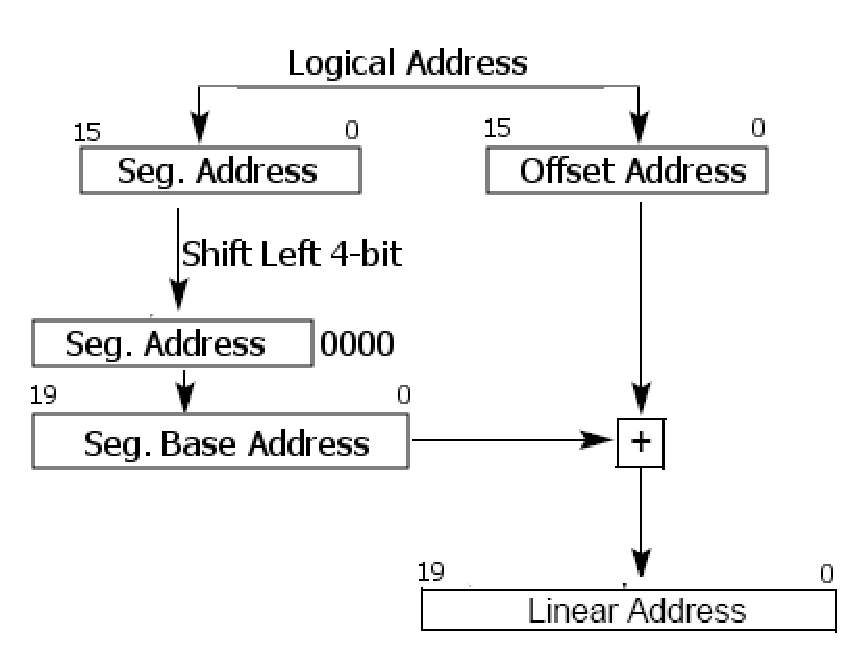
\includegraphics[width=.48\textwidth,keepaspectratio]{rm_addr}%
\label{rm_addr}}
\hfil
\subfloat[保护模式寻址模型]{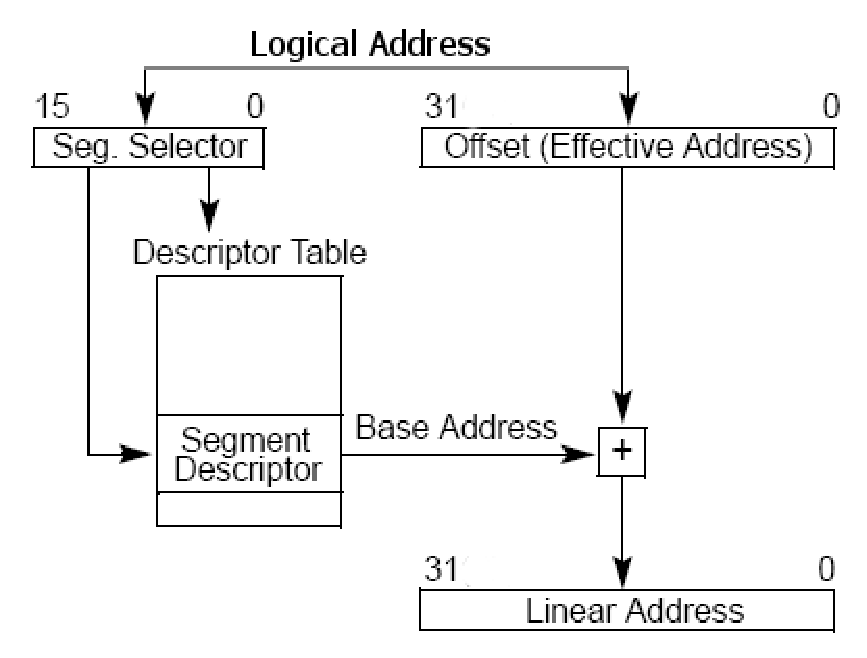
\includegraphics[width=.48\textwidth,keepaspectratio]{protected_seg}%
\label{protected_seg}}}
\caption{实模式与保护模式寻址模型比较}
\label{real_vs_pro}
\end{figure*}

一般情况下,段地址会被放在四个段寄存器中,即:代码段~CS,数据段~DS,堆栈段~SS~和附加段~ES~寄存器。这样在加载数据或者控制程序运行的时候,只需要一个偏移量参数,CPU~会自动用对应段的起始地址加上偏移量参数来得到需要的地址。(后继~CPU~又加上了两个段寄存器~FS~和~GS~,不过使用方式是基本一样的。)

由此可见,实模式的寻址模式是很简单的,就是用两个~16~位逻辑地址(段地址:偏移地址)组合成一个~20~位物理地址,而保护模式的寻址方式就要稍微复杂一点了。

\BOXED{0.9\textwidth}{
Intel~的~CPU~在保护模式下是可以选择打开分页机制的,但为了简单起见,我们先不开启分页机制,所以下面的讲解针对只有分段机制的保护模式展开。
}

在保护模式下,每个单元的物理地址仍然是由逻辑地址表示,但是这个逻辑地址不再由(段地址:偏移地址)组成了,而是由(段选择子:偏移地址)表示。这里的偏移地址也变成了~32~位的,所以段空间也比实模式下大得多。偏移地址的意思和实模式下并没有本质不同,但段地址的计算就要复杂一些了,如图~\ref{protected_seg}~所示。段基址(Segment Base Address)被存放在段描述符(Segment Descriptor)中,GDT(Global Descriptor Table,全局段选择子表)是保存着所有段选择子的信息,段选择子(Segment Selector)是一个指向某个段选择子的索引。

如图~\ref{protected_seg}~所示,当我们计算某个单元的物理地址时,只需要给出(段选择子:偏移地址),CPU~会从~GDT~中按照段选择子找到对应的段描述符,从段描述符中找出段基址,将段基址加上偏移量,就得到了该单元的物理地址。

\section{与保护模式初次会面}

介绍完了保护模式和实模式的不同,下面我们就尝试一下进入保护模式吧。在上一章我们已经实现了用启动扇区加载引导文件,所以这里我们就不用再去管启动扇区的事情了,下面的修改均在~loader.S~中进行。上一章的~loader.S~仅仅实现在屏幕的上方中间打印了一个~\code{L}~,下面我们的~loader.S~要进入保护模式来打印一些新东西。

首先,我们来理清一下应该如何进入保护模式:

\begin{enumerate}
  \item 我们需要一个~GDT。由于保护模式的寻址方式是基于~GDT~的,我们得自己写一个~GDT~数据结构并将其载入到系统中。
  \item 我们需要为进入保护模式作准备。由于保护模式和实模式运行方式不同,在进入保护模式之前,我们需要一些准备工作。
  \item 我们需要一段能在保护模式下运行的代码 demo,以提示我们成功进入了保护模式。
\end{enumerate}

下面我们就来一步步完成我们的第一个保护模式~loader~。

\subsection{GDT~数据结构}

要写~GDT,首先得了解~GDT~的数据结构。GDT~实际上只是一个存储段描述符的线性表(可以理解成一个段描述符数组),对它的要求是其第一个段描述符置为空,因为处理机不会去处理第一个段描述符,所以理解~GDT~的数据结构难点主要在于理解段描述符的数据结构。

段描述符主要用来为处理机提供段位址,段访问控制和状态信息。图~\ref{seg_desc}~显示了一个基本的段描述符结构:

\FIG{段描述符}{seg_desc}{.9\textwidth}

看到上面那么多内容,是不是感觉有点儿恐怖啊!其实简单的来看,我们现在最关注的是段基址,就是图~\ref{seg_desc}~中标记为~Base~的部分。可以看到,段基址在段描述符中被分割为三段存储,分别是:Base 31:24, Base 23:16, Base Address 15:0,把这三段拼起来,我们就得到了一个~32~位的段基址。

有了段基址,就需要有一个界限来避免程序跑丢发生段错误,这个界限就是图~\ref{seg_desc}~中标记为~Limit~的部分,将~Seg. Limit 19:16~和~Segment Limit 15:0~拼起来我们就得到了一个~20~位的段界限,这个界限就是应该是段需要的长度了。

下面还要说的就是那个~D/B Flag~,D/B~代表~Default Operation Size~,0~代表~16~位的段,1~代表~32~位的段。为了充分利用~CPU~,我们当然要设置为~32~位模式了。剩下那些乱七八糟的~Flag~呢,无非就是提供段的属性(代码段还是数据段?只读还是读写?),我们将在第~\ref{CHpm_desattr}~节为大家详细介绍。

这些东西那么乱,难道要每次一点儿一点儿地计算吗?放心,程序员自有办法,请看下面的程序:

\VerbatimInput[fontfamily=tt,fontsize=\footnotesize,frame=lines, framerule=0.4mm, numbers=left, numbersep=3pt, tabsize=2, firstline=56, lastline=70]{../src/chapter3/1/pm.h}
\codecaption{自动生成段描述符的宏定义(节自 chapter3/1/pm.h)}\label{CHpm_descm}

图~\ref{CHpm_descm}~中所示,就是自动生成段描述符的汇编宏定义。我们只需要给宏~Descriptor~三个参数:Base(段基址), Limit(段界限[段长度]), Attr(段属性),Descriptor~就会自动将三者展开放到段描述符中对应的位置。看看我们在程序中怎么使用这个宏:

\VerbatimInput[fontfamily=tt,fontsize=\footnotesize,frame=lines, framerule=0.4mm, numbers=left, numbersep=3pt, tabsize=2, firstline=21, lastline=26]{../src/chapter3/1/loader.S}
\codecaption{自动生成段描述符的宏使用示例(节自 chapter3/1/loader.S)}\label{CHpm_descmu}

图~\ref{CHpm_descmu}~中,就利用~Descriptor~宏生成了三个段描述符,形成了一个~GDT。注意到没有,第一个段描述符是空的(参数全为~0)。这里~LABEL\_DESC\_CODE32~的段基址为~0~是因为我们无法确定它的准确位置,它将在运行期被填入。

有人可能会产生疑问,段基址和段界限什么意思我们都知道了,那段属性怎么回事呢?~DA\_C, DA\_32, DA\_DRW~都是什么东西啊?是这样的,为了避免手动一个一个置段描述符中的~Flag~,我们预先定义了一些常用属性,用的时候只需要将这些属性加起来作为宏~Descriptor~的参数,就能将段描述符中的所有~flag~置上(记得~C~语言中~fopen~的参数吗?)。这些属性的定义如下(没必要细看,用的时候再找即可):

\VerbatimInput[fontfamily=tt,fontsize=\footnotesize,frame=lines, framerule=0.4mm, numbers=left, numbersep=3pt, tabsize=2, firstline=11, lastline=55]{../src/chapter3/1/pm.h}
\codecaption{预先设置的段属性(节自 chapter3/1/pm.h)}\label{CHpm_segattr}

\subsection{保护模式下的~demo}

为什么把这节提前到第~\ref{CHpm_secloadgdt}~节前讲呢?因为要写入~GDT~正确的段描述符,首先要知道段的信息,我们就得先准备好这个段:

\VerbatimInput[fontfamily=tt,fontsize=\footnotesize,frame=lines, framerule=0.4mm, numbers=left, numbersep=3pt, tabsize=2, firstline=83, lastline=99]{../src/chapter3/1/loader.S}
\codecaption{第一个在保护模式下运行的 demo(节自 chapter3/1/loader.S)}\label{CHpm_demo1}

其实这个段的作用很简单,通过操纵视频段数据,在屏幕中间打印一个红色的"P"(和我们前面使用~BIOS~中断来打印字符的方式有所不同)。

\subsection{加载~GDT} \label{CHpm_secloadgdt}

GDT~所需要的信息我们都知道了,GDT~表也通过图~\ref{CHpm_descmu}~中的代码实现了。那么,我们应该向~GDT~中填入缺少的信息,然后载入~GDT~了。将~GDT~载入处理机是用~\code{lgdt}~汇编指令实现的,但是~\code{lgdt}~指令需要存放~GDT~的基址和界限的指针作参数,所以我们还需要知道~GDT~的位置和~GDT~的界限:

\VerbatimInput[fontfamily=tt,fontsize=\footnotesize,frame=lines, framerule=0.4mm, numbers=left, numbersep=3pt, tabsize=2, firstline=22, lastline=63]{../src/chapter3/1/loader.S}
\codecaption{加载~GDT(节自 chapter3/1/loader.S)}\label{CHpm_loadgdt}

图~\ref{CHpm_loadgdt}~中~\code{GdtPtr}~所指,即为~GDT~的界限和基址所存放位置。某段描述符对应的~GDT~选择子,就是其段描述符相对于~GDT~基址的索引(在我们例子里~GDT~基址为~\code{LABEL\_GDT}~指向的位置)。这里需要注意的是,虽然我们在代码中写:

\begin{Command}
.set SelectorCode32, (LABEL_DESC_CODE32 - LABEL_GDT)
\end{Command}
但实际上段选择子在使用时需要右移~3~个位作为索引去寻找其对应的段描述符,段选择子的右侧~3~个位是为了标识~TI~和~RPL~的,如图~\ref{seg_selector}~所示,这点我们将在第~\ref{CHpm_ldt}~节和第~\ref{CHpm_desattr}~节中详细介绍。但是这里为什么能直接用地址相减得到段选择子呢?因为段选择子的大小是~8 bit~,用地址相减的话,最右侧三个位就默认置~0~了。

在图~\ref{CHpm_loadgdt}~中所示的代码,主要干了两件事:第一,将图~\ref{CHpm_demo1}~所示~demo~的段基址放入~GDT~中对应的段描述符中;第二,将~GDT~的基址放到~\code{GdtPtr}~所指的数据结构中,并加载~\code{GdtPtr}~所指的数据结构到~GDTR~寄存器中(使用~\code{lgdt}~指令)。

\subsection{进入保护模式}

进入保护模式前,我们需要将中断关掉,因为保护模式下中断处理的机制和实模式是不一样的,不关掉中断可能带来麻烦。使用~\code{cli}~汇编指令可以清除所有中断~flag。

由于实模式下仅有~20~条地址线:A0, A1, \ldots, A19,所以当我们要进入保护模式时,需要打开~A20~地址线。打开~A20~地址线有至少三种方法,我们这里采用~IBM~使用的方法,通常被称为:“Fast A20 Gate”,即修改系统控制端口~92h~,因为其端口的第~1~位控制着~A20~地址线,所以我们只需要将~0b00000010~赋给端口~92h~即可。

当前面两项工作完成后,我们就可以进入保护模式了。方法很简单,将~cr0~寄存器的第~0~位~PE~位置为~1~即可使~CPU~切换到保护模式下运行。

\VerbatimInput[fontfamily=tt,fontsize=\footnotesize,frame=lines, framerule=0.4mm, numbers=left, numbersep=3pt, tabsize=2, firstline=64, lastline=77]{../src/chapter3/1/loader.S}
\codecaption{进入保护模式(节自 chapter3/1/loader.S)}\label{CHpm_enablepm}

\subsection{特别的混合跳转指令}

虽然已经进入了保护模式,但由于我们的~CS~寄存器存放的仍然是实模式下~16~位的段信息,要跳转到我们的~demo~程序并不是那么简单的事情。因为~demo~程序是~32~位的指令,而我们现在仍然运行的是~16~位的指令。从~16~位的代码段中跳转到~32~位的代码段,不是一般的~near~或~far~跳转指令能解决得了的,所以这里我们需要一个特别的跳转指令。在这条指令运行之前,所有的指令都是~16~位的,在它运行之后,就变成~32~位指令的世界。

在~Intel~的手册中,把这条混合跳转指令称为~far jump(ptr16:32)~,在~NASM~手册中,将这条指令称为~Mixed-Size Jump~,我们就沿用~NASM~的说法,将这条指令称为混合字长跳转指令。NASM~提供了这条指令的汇编语言实现:
\begin{Command}
jmp dword 0x1234:0x56789ABC
\end{Command}
NASM~的手册中说~GAS~没有提供这条指令的实现,我就用~.byte~伪代码直接写了二进制指令:
\begin{Command}
/* Mixed-Size Jump. */
.2byte  0xea66
.4byte  0x00000000
.2byte  SelectorCode32
\end{Command}
但是有位朋友提醒我说现在的~GAS~已经支持混合字长跳转指令(如图~\ref{CHpm_mixedjmp}),看来~NASM~的手册好久没有维护喽~\smiley~。

\VerbatimInput[fontfamily=tt,fontsize=\footnotesize,frame=lines, framerule=0.4mm, numbers=left, numbersep=3pt, tabsize=2, firstline=77, lastline=82]{../src/chapter3/1/loader.S}
\codecaption{混合字长跳转指令(节自 chapter3/1/loader.S)}\label{CHpm_mixedjmp}

执行这条混合字长的跳转指令时,CPU~就会用段选择子~\code{SelectorCode32}~去寻找~GDT~中对应的段,由于段偏移是~0~,所以~CPU~将跳转到图~\ref{CHpm_demo1}~中~demo~程序的开头。为了方便阅读,整个~loader.S~的代码附在图~\ref{CHpm_loader1}~中:

\VerbatimInput[fontfamily=tt,fontsize=\footnotesize,frame=lines, framerule=0.4mm, numbers=left, numbersep=3pt, tabsize=2, firstline=1, lastline=99]{../src/chapter3/1/loader.S}
\codecaption{chapter3/1/loader.S (节自 chapter3/1/loader.S)}\label{CHpm_loader1}

\subsection{生成镜像并测试}

使用与第~\ref{CHsmall_test}~节完全相同的方法,我们可以将代码编译并将~LOADER.BIN~拷贝到镜像文件中。利用最新的镜像文件启动~VirtualBox~我们得到图~\ref{vb_run_5}~。

可以看到,屏幕的左侧中央打出了一个红色的~P~,这就是我们那个在保护模式下运行的简单~demo~所做的事情,这说明我们的代码是正确的。从实模式迈入保护模式,这只是一小步,但对于我们的操作系统来说,这是一大步。从此我们不必再被限制到~20~位的地址空间中,有了更大的自由度。

\FIG{第一次进入保护模式}{vb_run_5}{0.75\textwidth}

\section{段式存储}

如果您仔细阅读了图~\ref{protected_seg}~,您就会发现图中并未提到~GDT~,而是使用的~Descriptor Table(DT)~。这是因为对于~x86~架构的~CPU~来说,~DT~总共有两个:我们上节介绍过的~GDT~和下面要介绍的~LDT~。这两个描述符表构成了~x86 CPU~段式存储的基础。顾名思义,~GDT~作为全局的描述符表,只能有一个,而~LDT~作为局部描述符表,就可以有很多个,这也是以后操作系统给每个任务分配自己的存储空间的基础。

\subsection{LDT~数据结构} \label{CHpm_ldt}

\FIG{段选择子数据结构}{seg_selector}{0.6\textwidth}

事实上,~LDT~和~GDT~的差别非常小,~LDT~段描述符的数据结构和图~\ref{seg_desc}~所示是一样的。所不同的就是,~LDT~用指令~\code{lldt}~来加载,并且指向~LDT~描述符项的段选择子的~TI~位置必须标识为~1~,如图~\ref{seg_selector}~所示。这样,在使用~TI flag := 1~的段选择子时,操作系统才会从当前的~LDT~而不是~GDT~中去寻找对应的段描述符。

这里值得注意的一点是:GDT~是由线性空间里的地址定义的,即~\code{lgdt}~指令的参数是一个线性空间的地址;而~LDT~是由~GDT~中的一个段描述符定义的,即~\code{lldt}~指令的参数是~GDT~中的一个段选择子。这是因为在加载~GDT~之前寻址模式是实模式的,而加载~GDT~后寻址模式变成保护模式寻址,将~LDT~作为~GDT~中的段使用,也方便操作系统在多个~LDT~之间切换。

\subsection{段描述符属性} \label{CHpm_desattr}

我们在介绍图~\ref{seg_desc}~时,并没有完全介绍段描述符的各个~Flag~和可能的属性,这一小节就用来专门介绍段描述符的属性,按照图~\ref{seg_desc}~中的~Flag~从左向右的顺序:

\begin{itemize}
\item{\textbf{G}}: G(Granularity,粒度):如果~G flag~置为~0~,段的大小以字节为单位,段长度范围是~\code{1 byte$\sim$1 MB}~;如果~G flag~置为~1~,段的大小以~4 KB~为单位,段长度范围是~\code{4 KB $\sim$ 4 GB}~。
\item{\textbf{D/B}}:D/B(Default operation size/Default stack pionter size and/or upper Bound, 默认操作大小),其意思取决于段描述符是代码段、数据段或者堆栈段。该~flag~置为~0~代表代码段/数据段为~16~位的;置为~1~代表该段是~32~位的。
\item{\textbf{L}}:L(Long, 长),~L flag~是~IA-32e(Extended Memory 64 Technology)~模式下使用的标志。该~flag~置为~1~代表该段是正常的~64~位的代码段;置为~0~代表在兼容模式下运行的代码段。在~IA-32~架构下,该位是保留位,并且永远被置为~0~。
\item{\textbf{AVL}}:保留给操作系统软件使用的位。
\item{\textbf{P}}:P(segment-Present,段占用?) flag~用于标志段是否在内存中,主要供内存管理软件使用。如果~P flag~被置为~0~,说明该段目前不在内存中,该段指向的内存可以暂时被其它任务占用;如果~P flag~被置为~1~,说明该段在内存中。如果~P flag~为~0~的段被访问,处理机会产生一个~segment-not-present(\#NP)~异常。
\item{\textbf{DPL}}:DPL(Descriptor Privilege Level)域标志着段的优先级,取值范围是从~0$\sim$3(2-bit)~,0~代表着最高的优先级。关于优先级的作用,我们将在下节讨论。
\item{\textbf{S}}:S(descriptor type) flag~标志着该段是否系统段:置为~0~代表该段是系统段;置为~1~代表该段是代码段或者数据段。
\item{\textbf{Type}}:Type~域是段描述符里最复杂的一个域,而且它的意义对于代码/数据段描述符和系统段/门描述符是不同的,下面我们用两张表来展示当~Type~置为不同值时的意义。

表~\ref{code_data_types}~所示即为代码/数据段描述符的所有~Type~可能的值(0-15, 4-bit)以及对应的属性含意,表~\ref{sys_gate_types}~所示为系统段/门描述符的~Type~可能的值以及对应的属性含意。这两张表每个条目的内容是自明的,而且我们在后面的讨论中将不止一次会引用这两张表的内容,所以这里对每个条目暂时不加详细阐述。

\begin{center}\begin{longtable}{c|c|c|c|c|c|l}
\caption[]{代码/数据段描述符的~Type~属性列表}\label{code_data_types}\\
\hline
\multicolumn{5}{c|}{\textbf{Type Field}} & \textbf{Descriptor Type} & \textbf{Description}\bigstrut\\
\cline{1-5}
\textbf{Decimal} & \textbf{11} & \textbf{10} & \textbf{9} & \textbf{8} & & \\
        &    &  \textbf{E} & \textbf{W} & \textbf{A} & & \\
\hline
0 & 0 & 0 & 0 & 0 & Data & Read-Only\\
1 & 0 & 0 & 0 & 1 & Data & Read-Only, Accessed\\
2 & 0 & 0 & 1 & 0 & Data & Read/Write\\
3 & 0 & 0 & 1 & 1 & Data & Read/Write, Accessed\\
4 & 0 & 1 & 0 & 0 & Data & Read-Only, Expand-down\\
5 & 0 & 1 & 0 & 1 & Data & Read-Only, Expand-down, Accessed\\
6 & 0 & 1 & 1 & 0 & Data & Read/Write, Expand-down\\
7 & 0 & 1 & 1 & 1 & Data & Read/Write, Expand-down, Accessed\\
\hline
        &    &  \textbf{C} & \textbf{R} & \textbf{A} & & \\
\hline
8 & 1 & 0 & 0 & 0 & Code & Execute-Only\\
9 & 1 & 0 & 0 & 1 & Code & Execute-Only, Accessed\\
10 & 1 & 0 & 1 & 0 & Code & Execute/Read\\
11 & 1 & 0 & 1 & 1 & Code & Execute/Read, Accessed\\
12 & 1 & 1 & 0 & 0 & Code & Execute-Only, Conforming\\
13 & 1 & 1 & 0 & 1 & Code & Execute-Only, Conforming, Accessed\\
14 & 1 & 1 & 1 & 0 & Code & Execute/Read-Only, Conforming\\
15 & 1 & 1 & 1 & 1 & Code & Execute/Read-Only, Conforming, Accessed\\
\hline
\end{longtable}\end{center}

\begin{center}\begin{longtable}{c|c|c|c|c|l}
\caption[]{系统段/门描述符的~Type~属性列表}\label{sys_gate_types}\\
\hline
\multicolumn{5}{c|}{\textbf{Type Field}} & \textbf{Description}\bigstrut\\
\hline
\textbf{Decimal} & \textbf{11} & \textbf{10} & \textbf{9} & \textbf{8} & \textbf{32-Bit Mode}\\
\hline
0 & 0 & 0 & 0 & 0 & Reserved\\
1 & 0 & 0 & 0 & 1 & 16-bit TSS(Available)\\
2 & 0 & 0 & 1 & 0 & LDT\\
3 & 0 & 0 & 1 & 1 & 16-bit TSS(Busy)\\
4 & 0 & 1 & 0 & 0 & 16-bit Call Gate\\
5 & 0 & 1 & 0 & 1 & Task Gate\\
6 & 0 & 1 & 1 & 0 & 16-bit Interrupt Gate\\
7 & 0 & 1 & 1 & 1 & 16-bit Trap Gate\\
8 & 1 & 0 & 0 & 0 & Reserved\\
9 & 1 & 0 & 0 & 1 & 32-bit TSS(Available)\\
10 & 1 & 0 & 1 & 0 & Reserved\\
11 & 1 & 0 & 1 & 1 & 32-bit TSS(Busy)\\
12 & 1 & 1 & 0 & 0 & 32-bit Call Gate\\
13 & 1 & 1 & 0 & 1 & Reserved\\
14 & 1 & 1 & 1 & 0 & 32-bit Interrupt Gate\\
15 & 1 & 1 & 1 & 1 & 32-bit Trap Gate\\
\hline
\end{longtable}\end{center}

\end{itemize}

\subsection{使用~LDT~}

从目前的需求来看,对~LDT~并没有非介绍不可的理由,但是理解~LDT~的使用,对理解段式存储和处理机多任务存储空间分配有很大的帮助。所以我们在下面的代码中实现几个简单的例子:一,建立~32~位数据和堆栈两个段并将描述符添加到~GDT~中;二,添加一段简单代码,并以其段描述符为基础建立一个~LDT;三,在~GDT~中添加~LDT~的段描述符并初始化所有~DT~;四,进入保护模式下运行的~32~位代码段后,加载~LDT~并跳转执行~LDT~中包含的代码段。

首先,建立~32~位全局数据段和堆栈段,并将其描述符添加到~GDT~中:

\VerbatimInput[fontfamily=tt,fontsize=\footnotesize,frame=topline, framerule=0.4mm, numbers=left, numbersep=3pt, tabsize=2, firstline=50, lastline=62]{../src/chapter3/2/loader.S}
\VerbatimInput[fontfamily=tt,fontsize=\footnotesize,frame=bottomline, framerule=0.4mm, numbers=left, numbersep=3pt, tabsize=2, firstline=22, lastline=41]{../src/chapter3/2/loader.S}
\codecaption{32~位全局数据段和堆栈段,以及对应的~GDT~结构(节自 chapter3/2/loader.S)}\label{CHpm_add_ds}

在图~\ref{CHpm_add_ds}~中,我们首先建立了一个全局的数据段,并在数据段里放置了两个字符串,分别用来进入保护模式后和跳转到~LDT~指向的代码段后作为信息输出。然后又建立了一个全局的堆栈段,为堆栈段预留了~512~字节的空间,并将栈顶设置为距栈底~511~字节处。然后与上节介绍的类似,将数据段和堆栈段的段描述符添加到~GDT~中,并设置好对应的段选择子。

要注意到数据段、堆栈段和代码段的段描述符属性不尽相同。数据段的段描述符属性是~\code{DA\_DRW}~,回忆我们前面~pm.h~的内容(图~\ref{CHpm_segattr}~),~\code{DA\_DRW}~的内容是~\code{0x92},用二进制就是~\code{10010010},其后四位就对应着图~\ref{code_data_types}~中的第二~2(0010)~项,说明这个段是可读写的数据段;前四位对应着~\code{P|DPL|S}~三个~flag~,即~\code{P:1, DPL:00, S:1}~,与第~\ref{CHpm_desattr}~节结合理解,意思就是该段在内存中,为最高的优先级,非系统段。所以我们可以看到~pm.h~中的各个属性变量定义,就是将二进制的属性值用可理解的变量名表示出来,在用的时候直接加上变量即可。

同理我们也可以分别来理解~GDT~中堆栈段和代码段描述符的属性定义。因为不同类型的属性使用的是段描述符中不同的位,所以不同类型的属性可以直接相加得到复合的属性值,例如堆栈段的~\code{(DA\_DRWA + DA\_32)}~,其意思类似于~\code{C++}~中~\code{fstream}~打开文件时可以对模式进行算术或(\code{ios\_base::in | ios\_base::out})来得到复合参数。

其次,添加一段简单的代码,并以其描述符为基础建立一个~LDT:

\VerbatimInput[fontfamily=tt,fontsize=\footnotesize,frame=topline, framerule=0.4mm, numbers=left, numbersep=3pt, tabsize=2, firstline=114, lastline=140]{../src/chapter3/2/loader.S}
\VerbatimInput[fontfamily=tt,fontsize=\footnotesize,frame=bottomline, framerule=0.4mm, numbers=left, numbersep=3pt, tabsize=2, firstline=42, lastline=49]{../src/chapter3/2/loader.S}
\codecaption{32~位代码段,以及对应的~LDT~结构(节自 chapter3/2/loader.S)}\label{CHpm_build_ldt}

\code{LABEL\_CODEA}~就是我们为~LDT~建立的简单代码段,其作用就是操作显存在屏幕的第~12~行开始用红色的字打印出偏移~\code{OffsetLDTMessage}~指向的全局数据段中的字符串。下面就是以~\code{LABEL\_CODEA}~为基础建立的~LDT~,从~LDT~的结构来说,与~GDT~没有区别,但是我们不用像~\code{GdtPtr}~再建立一个~\code{LdtPtr}~,因为~LDT~实际上是在~GDT~中定义的一个段,不用实模式的线性地址表示。

LDT~的选择子是与~GDT~选择子有明显区别的,图~\ref{seg_selector}~清楚地解释了这一点,所以指向~LDT~的选择子都应该将~TI~位置~1~,在图~\ref{CHpm_build_ldt}~的最后一行也实现了这一操作。

第三,在~GDT~中添加~LDT~的段描述符(在图~\ref{CHpm_add_ds}~中我们已经能看到在~GDT~中添加好了~LDT~的段描述符),初始化所有段描述符。由于初始化段描述符属于重复性工作,我们在~pm.h~中添加一个汇编宏~\code{InitDesc}~来帮我们做这件事情。

\VerbatimInput[fontfamily=tt,fontsize=\footnotesize,frame=lines, framerule=0.4mm, numbers=left, numbersep=3pt, tabsize=2, firstline=84, lastline=96]{../src/chapter3/2/pm.h}
\codecaption{自动初始化段描述符的宏代码(节自 chapter3/2/pm.h)}\label{CHpm_initdesc}

\VerbatimInput[fontfamily=tt,fontsize=\footnotesize,frame=lines, framerule=0.4mm, numbers=left, numbersep=3pt, tabsize=2, firstline=63, lastline=112]{../src/chapter3/2/loader.S}
\codecaption{在实模式代码段中初始化所有段描述符(节自 chapter3/2/loader.S)}\label{CHpm_init_dts}

初始化各个段描述符的方式与上一节介绍的初始化~GDT~描述符的方式没有什么本质不同,因为属性都已经预设好,运行时只需要将段地址填入描述符中的地址域即可,代码都是重复的。我们引入宏~\code{InitDesc}的帮助,能大大缩短代码长度,增强代码的可读性。

第四,进入保护模式下运行的~32~位代码段后,加载~LDT~并跳转执行~LDT~中包含的代码段:

\VerbatimInput[fontfamily=tt,fontsize=\footnotesize,frame=lines, framerule=0.4mm, numbers=left, numbersep=3pt, tabsize=2, firstline=141, lastline=176]{../src/chapter3/2/loader.S}
\codecaption{在保护模式代码段中加载~LDT~并跳转执行~LDT~代码段(节自 chapter3/2/loader.S)}\label{CHpm_run_ldt}

在~\code{LABEL\_SEG\_CODE32}~中前几行,我们可以看到非常熟悉的汇编指令,和一般汇编程序开头初始化数据/代码/堆栈段寄存器的指令非常像,只不过这里赋给几个寄存器的参数都是段选择子,而不是一般的地址。该代码段剩下的内容和前面图~\ref{CHpm_build_ldt}~中~\code{LABEL\_CODEA}~一样,都是打印一个字符串,只不过这里选择在第~10~行(屏幕左侧中央)打印。

为了方便阅读,整个~loader.S~的代码附在图~\ref{CHpm_loader2}~中。

\VerbatimInput[fontfamily=tt,fontsize=\footnotesize,frame=lines, framerule=0.4mm, numbers=left, numbersep=3pt, tabsize=2]{../src/chapter3/2/loader.S}
\codecaption{chapter3/2/loader.S}\label{CHpm_loader2}

\subsection{生成镜像并测试}

使用与第~\ref{CHsmall_test}~节完全相同的方法,我们可以将代码编译并将~LOADER.BIN~拷贝到镜像文件中。利用最新的镜像文件启动~VirtualBox~我们得到图~\ref{vb_run_6}~。

\FIG{第一次进入保护模式}{vb_run_6}{0.75\textwidth}

可以看到,该程序首先在屏幕左侧中央(第~10~行)打印出来~\code{"Welcome to protect mode!\^{}-\^{}"}~,这是由~GDT~中的~32~位代码段~\code{LABEL\_SEG\_CODE32}~打印出来的,标志着我们成功进入保护模式;然后在屏幕的第~12~行打印出来~\code{"Aha, you jumped into a LDT segment."}~,这个是由~LDT~中的~32~位代码段~\code{LABEL\_CODEA}~打印出来的,标志着~LDT~的使用正确。因为这两个字符串都是被存储在~32~位全局数据段中,这两个字符串的成功打印也说明在~GDT~中添加的数据段使用正确。

\subsection{段式存储总结}

段式存储和页式存储都是最流行的计算机内存保护方式。段式存储的含义简单来说就是先将内存分为各个段,然后再分配给程序供不同用途使用,并保证对各个段的访问互不干扰。x86~主要使用段寄存器(得到的段基址)~\code{+}~偏移量来访问段中数据,也简化了寻址过程。

在~x86~的初期实模式下就使用着非常简单的段式存储方式,如图~\ref{rm_addr}~所示,这种模式下分段主要是为了方便寻址和隔离,没有提供其它的保护机制。x86~保护模式下采用了更高级的段式存储方式:用全局和局部描述符表存储段描述符信息,使用段选择子表示各个段描述符,如图~\ref{protected_seg}~所示。

由于保护模式使用段描述符来保存段信息而不是像实模式一样直接使用段地址,在段描述符中就可以添加一些属性来限制对段的访问权限,如我们在第~\ref{CHpm_desattr}~节中讨论的那样。这样,通过在访问段时检查权限和属性,就能做到对程序段的更完善保护和更好的内存管理。

x86~使用全局描述符表(GDT)和局部描述符表(LDT)来实现不同需求下对程序段的控制,操作系统使用唯一的一个~GDT~来维护一些和系统密切相关的段描述符信息,为不同的任务使用不同的~LDT~来实现对多任务内存管理的支持,简化了任务切换引起的内存切换的难度。

\section{特权级}

\BOXED{0.9\textwidth}{
\danger\\ 如果您需要更详细的知识,也许您更愿意去读 Intel 的手册,本节内容主要集中在:\href{http://download.intel.com/design/processor/manuals/253668.pdf}{Intel\textregistered~64 and IA-32 Architectures Software Developer's Manual, Volume 3A: System Programming Guide}, 第~4~章.\enddanger
}

特权级是为了保护处理机资源而引入的概念。将同一个处理机上执行的不同任务赋予不同的特权级,可以控制该任务可以访问的资源,比如内存地址范围、输入输出端口、和一些特殊指令的使用。在~x86~体系结构中,共有~4~个特权级别,0~代表最高特权级,3~代表最低特权级。由于在~x86~体系结构中,n~级可以访问的资源均可以被~0~到~n~级访问,这个模式被称作~ring~模式,相应地我们也将~x86~的对应特权级称作~ring n。

现代的~PC~操作系统的内核一般工作在~ring 0~下,拥有最高的特权级,应用程序一般工作在~ring 3~下,拥有最低的优先级。虽然~x86~体系结构提供了~4~个特权级,但操作系统并不需要全部使用到这~4~个级别,可以根据需要来选择使用几个特权级。比如~Linux/Unix~和~Windows NT~,都是只使用了~0~级和~3~级,分别用于内核模式和用户模式;而~DOS~则只使用了~0~级。

为了实施对代码段和数据段的特权级检验,x86~处理机引入了以下三种特权级类型(请注意这里提到的特权级高低均为实际高低,而非数值意义上的高低):

\begin{itemize}
\item{\textbf{CPL(Current Privilege Level)}}:当前特权级,存储在~CS~和~SS~的~0, 1~位。它代表当前执行程序或任务的特权级,通常情况下与当前执行指令所在代码段的~DPL~相同。当程序跳转到不同特权级的代码段时,CPL~会随之修改。当访问一致代码段(Conforming Code Segment)时,对~CPL~的处理有些不同。一致代码段可以被不高于(数值上大于等于)该段~DPL~的特权级代码访问,但是,CPL~在访问一致代码段时不会跟随~DPL~的变化而更改。
\item{\textbf{DPL(Descriptor Privilege Level)}}:描述符特权级,定义于段描述符或门描述符中的~DPL~域(见图~\ref{seg_desc}),它限制了可以访问此段资源的特权级别。根据被访问的段或者门的不同,DPL~的意义也不同:
  \begin{itemize}
  \item{\textbf{数据段}}:数据段的~DPL~限制了可以访问该数据段的最低特权级。假如数据段的~DPL~为~1,那么只有~CPL~为~0,1~的程序才能访问该数据段。
  \item{\textbf{非一致代码段(不使用调用门)}}:非一致代码段就是一般的代码段,它的~DPL~表示可以访问该段的特权级,程序或者任务的特权级必须与该段的~DPL~完全相同才可以访问该段。
  \item{\textbf{调用门}}:调用门的~DPL~限制了可以访问该门的最低特权级,与数据段~DPL~的意思一样。
  \item{\textbf{一致代码段和使用调用门访问的非一致代码段}}:这种代码段的~DPL~表示可以访问该段的最高特权级。假如一致代码段的~DPL~是~2,那么~CPL~为~0,1~的程序就无法访问该段。
  \item{\textbf{TSS(Task State Segment)}}:任务状态段的~DPL~表示可以访问该段的最低特权级,与数据段~DPL~的意思一样。
  \end{itemize}
比如一个数据段的~DPL~为~1~,那么只有当前特权级(CPL)为~0~或~1~的程序可以访问该段。
\item{\textbf{RPL(Requested Privilege Level)}}:请求特权级,定义于段选择子的~RPL~域中(见图~\ref{seg_selector})。它限制了这个选择子可访问资源的最高特权级。比如一个段选择子的~RPL~为~3~,那么使用这个段选择子只能访问~DPL~为~3~或者~4~的段,即使使用这个段选择子的程序当前特权级(CPL)为~0~。就是说,$\max{(CPL, RPL)}\le DPL$~才被允许访问该段,即当~CPL~小于~RPL~时,RPL~起决定性作用,反之亦然。使用~RPL~可以避免特权级高的程序代替应用程序访问该应用程序无权访问的段。比如在系统调用时,应用程序调用系统过程,虽然系统过程的优先级高($CPL=0$),但是被调用的系统过程仍然无法访问特权级高于应用程序的段($DPL<RPL=4$),就避免了可能出现的安全问题。
\end{itemize}

在将段描述符对应的段选择子加载到段寄存器时,处理机通过将~CPL, 段选择子的~RPL~和该段的~DPL~相比较,来判断程序是否有权访问另外一个段。如果~$CPL>\max{(RPL, DPL)}~$,或者$\max{(CPL, RPL)}>DPL$,那么该访问就是不合法的,处理机就会产生一个常规保护异常(\texttt{\#}GP, General Protection Exception)。

\subsection{不合法的访问请求示例}

我们来看一个不合法的访问请求的例子,在上一节的~loader.S~中把~\code{LABEL\_DESC\_DATA}~对应的描述符的~\code{DPL}~设置为~1,然后将该数据段对应的段选择子的~RPL~设置为~3,即修改以下两行:
\begin{Command}
LABEL_DESC_DATA:    Descriptor        0,      (DataLen - 1), (DA_DRW + DA_DPL1)
.set    SelectorData,   (LABEL_DESC_DATA   - LABEL_GDT + SA_RPL3)
\end{Command}

\FIGFIX{虚拟机出现异常,黑屏}{vb_run_7}{0.75\textwidth}

\FIGFIX{虚拟退出后~VBox~主窗口显示~Abort}{vb_main_4}{0.75\textwidth}

再~\code{make, sudo make copy},用~VirtualBox~加载生成的镜像运行一下,就会发现虚拟机黑屏一会儿就会退出(如图~\ref{vb_run_7}),然后~VirtualBox~主窗口中显示该虚拟机~Aborted(如图~\ref{vb_main_4})。这是因为我们违反特权级的规则,使用~RPL=3~的选择子去访问~DPL=1~的段,这个不合法的访问请求引起处理机产生常规保护异常(\texttt{\#}GP)。而我们又没有准备对应的异常处理模块,当处理机找不到异常处理程序时就只好退出了。


\subsection{控制权转移的特权级检查}

在将控制权从一个代码段转移到另一个代码段之前,目标代码段的段选择子必须被加载到~CS~中。处理器在这个过程中会查看目标代码段的段描述符以及对其界限、类型(见图~\ref{seg_desc})和特权级进行检查。如果没有错误发生,CS~寄存器会被加载,程序控制权被转移到新的代码段,从~EIP~指示的位置开始运行。

JMP, CALL, RET, SYSENTER, SYSEXIT, INT n~和~IRET~这些指令,以及中断和异常机制都会引起程序控制权的转移。

JMP~和~CALL~指令可以实现以下~4~种形式的转移:

\begin{itemize}
\item 目标操作数包含目标代码段的段选择子。
\item 目标操作数指向一个包含目标代码段段选择子的调用门描述符。
\item 目标操作数指向一个包含目标代码段段选择子的任务状态段。
\item 目标操作数指向一个任务门,这个任务门指向一个包含目标代码段段选择子的任务状态段。
\end{itemize}

下面两个小节将描述前两种转移的实现方法,后两种控制权转移方法我们将在用到时再进行解释。

\subsubsection{用~JMP~或~CALL~直接转移}

用~JMP, CALL~和~RET~指令在段内进行近跳转并没有特权级的变化,所以对这类转移是不进行特权级检查的;用~JMP, CALL~和~RET~在段间进行远跳转涉及到其它代码段,所以要进行特权级检查。

对不通过调用门的直接转移来说,又分为两种情形:

\begin{itemize}
\item{访问非一致代码段}:当目标是非一致代码段时(目标段段描述符的~C flag~为~0~,见图~\ref{code_data_types}),特权级检查要求调用者的~CPL~与目标代码段的~DPL~相等,而且调用者使用的目标代码段段选择子的~RPL~必须小于等于目标代码段的~DPL。我们之前的代码都属于这种情形,其中~$CPL=DPL=RPL=0$。
\item{访问一致代码段}:当目标是一致代码段时(目标段段描述符的~C flag~为~1~,见图~\ref{code_data_types}),特权级检查要求~$CPL \ge DPL$,RPL~不被检查,而且转移时并不修改~CPL。
\end{itemize}

总的来说,通过~JMP~和~CALL~实行的都是一般的转移,最多从低特权级转移到高特权级的一致代码段,CPL~总是不变的。

\subsection{使用调用门转移}

调用门是~x86~体系结构下用来控制程序在不同特权级间转移的一种机制。它的目的是使低特权级的代码能够调用高特权级的代码,这一机制在使用了内存保护和特权级机制的现代操作系统中非常有用,因为它允许应用程序在操作系统控制下安全地调用内核例程或者系统接口。

\FIG{调用门描述符}{callgate_desc}{.9\textwidth}

门其实也是一种描述符,和段描述符类似。调用门描述符的数据结构如图~\ref{callgate_desc}~所示。其实看起来这个调用门描述符的数据结构要比段描述符简单一些,至少从它的属性来说,没有段描述符多。我们仍然只关注最重要的部分:首先是段选择子(Segment Selector),指定了通过这个调用门访问的代码段;其次是段偏移量(Offset in Segment),指定了要访问代码段中的某个入口偏移;描述符特权级(DPL),代表此门描述符的特权级;P,代表此调用门是否可用;参数计数(Param. Count)记录了如果发生栈切换的话,有多少个选项参数会在栈间拷贝。

简单来说,调用门描述了由一个段选择子和一个偏移所指定的目标代码段中的一个地址,程序通过调用门将转移到这个地址。下面我们通过一个简单的例子来介绍一下调用门的基本使用方法。

\subsubsection{简单的调用门转移举例}

为了使用调用门,我们首先要给出一个目标段,然后用该目标段的信息初始化调用门的门描述符,最后用调用门的门选择子实现门调用。

添加一个目标段我们已经做过很多次,非常简单。首先在上一节~loader.S~最后添加一个打印一个字符的代码段~\code{LABEL\_SEG\_CODECG},接着将该段的段描述符~\code{LABEL\_DESC\_CODECG}~添加到~GDT~中,然后为该段准备一个段选择子~\code{SelectorCodeCG},最后加入初始化该段描述符的代码:

\VerbatimInput[fontfamily=tt,fontsize=\footnotesize,frame=topline, framerule=0.4mm, numbers=left, numbersep=3pt, tabsize=2, firstline=197, lastline=211]{../src/chapter3/3/loader.S}
\VerbatimInput[fontfamily=tt,fontsize=\footnotesize,frame=none, framerule=0.4mm, numbers=left, numbersep=3pt, tabsize=2, firstline=28, lastline=29]{../src/chapter3/3/loader.S}
\VerbatimInput[fontfamily=tt,fontsize=\footnotesize,frame=none, framerule=0.4mm, numbers=left, numbersep=3pt, tabsize=2, firstline=43, lastline=44]{../src/chapter3/3/loader.S}
\VerbatimInput[fontfamily=tt,fontsize=\footnotesize,frame=bottomline, framerule=0.4mm, numbers=left, numbersep=3pt, tabsize=2, firstline=92, lastline=94]{../src/chapter3/3/loader.S}
\codecaption{添加调用门的目标段(节自 chapter3/3/loader.S)}\label{CHpm_codecg}

总的来看,~\code{LABEL\_SEG\_CODECG}~指向的这个段和我们以前为了打印程序运行结果所使用的段没有本质不同,为了简单起见,这里我们仅仅让它打印一个字符~\code{'C'}~就返回。

用目标代码段~\code{LABEL\_SEG\_CODECG}~的信息初始化调用门的门描述符~\code{LABEL\_CG\_TEST},以及门选择子~\code{SelectorCGTest}。与汇编宏~\code{Descriptor}~类似,我们这里使用汇编宏~\code{Gate}~来初始化门描述符,宏~\code{Gate}~的定义可以在头文件~\code{pm.h}~中找到:

\VerbatimInput[fontfamily=tt,fontsize=\footnotesize,frame=lines, framerule=0.4mm, numbers=left, numbersep=3pt, tabsize=2, firstline=71, lastline=82]{../src/chapter3/3/pm.h}
\codecaption{汇编宏~Gate~定义(节自 chapter3/3/pm.h)}\label{CHpm_cg_gate}

\VerbatimInput[fontfamily=tt,fontsize=\footnotesize,frame=topline, framerule=0.4mm, numbers=left, numbersep=3pt, tabsize=2, firstline=29, lastline=33]{../src/chapter3/3/loader.S}
\VerbatimInput[fontfamily=tt,fontsize=\footnotesize,frame=bottomline, framerule=0.4mm, numbers=left, numbersep=3pt, tabsize=2, firstline=43, lastline=45]{../src/chapter3/3/loader.S}
\codecaption{设置调用门描述符及选择子(节自 chapter3/3/loader.S)}\label{CHpm_cg_test}

我们可以看到,宏~\code{Gate}~的四个参数分别为:段选择子、偏移量、参数计数和属性,它们在存储空间中的分布与图~\ref{callgate_desc}~中介绍相同。由于这个例子仅仅介绍调用门的简单使用,并不涉及特权级切换,所以也不发生栈切换,这里我们将参数计数设置为~0;门描述符的属性为~\code{(DA\_386CGate + DPL)}~,表明它是一个调用门(属性定义见图~\ref{CHpm_descm}),DPL~为~0~,与我们一直使用的特权级相同;目标代码段选择子是~\code{SelectorCodeCG}~,偏移是~0~,所以如果该调用门被调用,将转移到目标代码段的开头,即~\code{LABEL\_SEG\_CODECG}~处开始执行。

使用远调用~lcall~指令调用该调用门的门选择子~\code{SelectorCGTest}:

\VerbatimInput[fontfamily=tt,fontsize=\footnotesize,frame=lines, framerule=0.4mm, numbers=left, numbersep=3pt, tabsize=2, firstline=185, lastline=190]{../src/chapter3/3/loader.S}
\codecaption{调用门选择子(节自 chapter3/3/loader.S)}\label{CHpm_cg_call1}

由于对调用门的调用往往涉及到段间转移,所以我们通常使用~gas~的~lcall~远跳转指令和~lret~远返回指令进行调用和返回。

这样我们就完成了使用调用门进行简单控制权转移的代码,~\code{make, sudo make copy}~之后,用~VBox~虚拟机载入生成的镜像,运行结果如图~\ref{vb_run_8}~所示。由于我们仅仅是在加载~LDT~之前添加了一个门调用,而且门调用的目标段在屏幕的第~11~行第~0~列打印了一个~\code{'C'}~后就返回到了调用处,所以加载~LDT~的代码继续运行,就是图中所示结果。

\FIG{使用调用门进行简单的控制权转移}{vb_run_8}{0.75\textwidth}

\subsubsection{涉及特权级变化的调用门转移}

在上面例子中我们只是使用调用门取代了传统的直接跳转方式,并没有涉及到特权级的变化。显然调用门不是用来做这种自找麻烦的事情的,其设计的主要目的是实现从低特权级代码跳转到高特权级的非一致代码的功能。

在使用调用门进行转移时,处理机会使用四个特权级值来检查控制权的转移是否合法:

\begin{enumerate}
\item CPL:当前特权级;
\item RPL:调用门选择子的请求特权级;
\item DPL:调用门描述符的描述符特权级;
\item DPL:目标代码段的段描述符特权级。
\end{enumerate}

使用~CALL~或者~JMP~指令访问调用门进行控制权转移时,特权级检查的规则有所不同,如表~\ref{callgate_rules}~所示:

\begin{center}\begin{longtable}{|l|l|}
\caption[]{调用门特权级检查规则}\label{callgate_rules}\\
\hline
\textbf{指令} & \textbf{特权级检查规则}\\
\hline
CALL & CPL $\le$ 调用门~DPL; RPL $\le$ 调用门~DPL\\
     & 目标段 DPL $\le$ CPL\\
\hline
JMP  & CPL $\le$ 调用门~DPL; RPL $\le$ 调用门~DPL\\
     & 当目标段是一致代码段时:目标段~DPL $\le$ CPL\\
     & 当目标段是非一致代码段时:目标段~DPL = CPL\\
\hline
\end{longtable}\end{center}

这张表内容虽然不多,但也不容易很快理解。这里我们应该着重看目标段~DPL~和~CPL~的比较,这才是调用门特权级检验的特点所在。总的来说,使用调用门需要目标段的~DPL~小于或等于~CPL~,意思就是要转移的目标段特权级高于当前特权级。这与我们在本节开头看到的一般转移的特权级检查有非常明显的不同。除此之外剩下的检查就是对调用门访问的检查了,这种特权级检查和访问一个数据段时进行的特权级检查的规则是一样的,我们已经熟知了。

我们已经了解了涉及特权级变化的调用门转移时处理机进行的特权级检查规则,但为了写一段从低特权级转移到高特权级的测试代码,我们仍然需要处理一个问题:如何从高特权级转移到低特权级?因为我们之前的代码一直运行在~ring 0~特权级上,要实现从低到高的转移,首先要从高特权级转到低特权级。

其实思想很简单,既然~CALL~指令能从低特权级转移到高特权级,自然而然地~RET~指令能从高特权级返回低特权级。我们只需要~hack~一下~RET~指令的使用方法即可(即用~RET~指令实现跳转到低特权级代码的功能)。

一般~CALL~和~RET~指令都是配合使用的,先用~CALL~跳转到目标地址,目标代码执行完后再用~RET~返回到~CALL~的下一条指令。为了从~ring 0~跳转到~ring 3~,我们并不使用~CALL~而直接执行~RET。为了使~RET~执行返回时不出错,我们需要为~RET~准备好返回时环境,就像通常执行~CALL~指令后处理机进行的工作一样。

那么执行~CALL~指令时处理机都进行了哪些工作呢?这是一个非常复杂的问题,我们将留待下个小节再详细介绍。但是在我们的例子里(即最简单的情况下),CALL~所做的就是将~SS, ESP, CS, EIP~这四个寄存器的值顺序压到栈里,这样在~RET~指令执行的时候,处理机从堆栈~pop~出~EIP, CS, ESP, SS~的值来恢复~CALL~指令执行后的处理机现场。所以为了使~RET~跳转到我们想要执行的代码段,我们只需要手动将~ring 3~目标代码段的对应的~SS, ESP, CS, EIP~值压到栈里即可。

下面开始准备这个~demo,仍旧是在上一节代码的基础上进行添加。首先,我们准备一个~ring 3~目标代码段和新栈:

\VerbatimInput[fontfamily=tt,fontsize=\footnotesize,frame=lines, framerule=0.4mm, numbers=left, numbersep=3pt, tabsize=2, firstline=224, lastline=238]{../src/chapter3/4/loader.S}
\codecaption{要运行在~ring 3~下的代码段(节自 chapter3/4/loader.S)}\label{CHpm_coder3}

\VerbatimInput[fontfamily=tt,fontsize=\footnotesize,frame=lines, framerule=0.4mm, numbers=left, numbersep=3pt, tabsize=2, firstline=73, lastline=76]{../src/chapter3/4/loader.S}
\codecaption{为~ring 3~代码段准备的新栈(节自 chapter3/4/loader.S)}\label{CHpm_stackr3}

这个代码段的功能就是在第~11~行第~1~列打印一个~3~字。

其次,添加新段的描述符和选择子,并添加初始化代码:

\VerbatimInput[fontfamily=tt,fontsize=\footnotesize,frame=topline, framerule=0.4mm, numbers=left, numbersep=3pt, tabsize=2, firstline=29, lastline=31]{../src/chapter3/4/loader.S}
\VerbatimInput[fontfamily=tt,fontsize=\footnotesize,frame=topline, framerule=0.4mm, numbers=left, numbersep=3pt, tabsize=2, firstline=47, lastline=49]{../src/chapter3/4/loader.S}
\codecaption{为~ring 3~代码段和堆栈段添加的描述符和选择子(节自 chapter3/4/loader.S)}\label{CHpm_coder3_desc}

\VerbatimInput[fontfamily=tt,fontsize=\footnotesize,frame=lines, framerule=0.4mm, numbers=left, numbersep=3pt, tabsize=2, firstline=105, lastline=109]{../src/chapter3/4/loader.S}
\codecaption{初始化~ring 3~代码段和堆栈段描述符的代码(节自 chapter3/4/loader.S)}\label{CHpm_coder3_init}

我们注意到,其实~ring 3~下的代码段和~ring 0~下的代码段的代码部分是没有任何区别的,区别在于它们的代码段描述符和选择子中所标明的特权级。我们将~ring 3~下的目标代码段和堆栈段的段描述符属性中加上~\code{DA\_DPL3}~,表明它们的段描述符特权级均为~3~;在它们的段选择子属性中加上~\code{SA\_RPL3}~,表明它们的段选择子请求特权级均为~3~。以上这两点限制了这个段只能在~ring 3~下运行。

准备好了两个段,我们将这两个段的信息作为~SS, ESP, CS, EIP~的内容依次压栈,然后再执行~lret~长返回指令,就能跳转到~ring 3~下运行目标代码段了:

\VerbatimInput[fontfamily=tt,fontsize=\footnotesize,frame=lines, framerule=0.4mm, numbers=left, numbersep=3pt, tabsize=2, firstline=191, lastline=199]{../src/chapter3/4/loader.S}
\codecaption{hack RET~指令进行实际的跳转}\label{CHpm_coder3_init}

这样,我们就完成了从高特权级代码(ring 0)跳转到低特权级代码(ring 3)的过程。像往常那样使用~make, sudo make copy~编译,用虚拟机加载镜像运行结果如图所示。

\end{document}
